%!TEX TS-program = pdflatex

%%%%%%%%%%%%%%%%%%%%%%%%%%%%%%%%%%%%%%%%%%%%%%%%%%%%%%%%%%%%%%%%%%%%%%%%%%%%
% BERT Vision : UC Berkeley MIDS - W266 NLP & Deep Learning
% MIDS Summer 2020, Section 1, Daniel Cer, PhD
% Final : BERT Vision
% Authors : Cristopher Benge (cris.benge@berkeley.edu)
%			William Casey King, PhD (cking@ischool.berkeley.edu)
%			Siduo "Stone" Jiang (siduojiang@ischool.berkeley.edu)
%%%%%%%%%%%%%%%%%%%%%%%%%%%%%%%%%%%%%%%%%%%%%%%%%%%%%%%%%%%%%%%%%%%%%%%%%%%%

%%%%%%%%%%%%%%%%%%%%%%%%%%%%%%%%%%%%%%%%%%%%%%%%%%%%%%%%%%%%%%%%%%%%%%%%%%%%
%%% PACKAGES
%%%%%%%%%%%%%%%%%%%%%%%%%%%%%%%%%%%%%%%%%%%%%%%%%%%%%%%%%%%%%%%%%%%%%%%%%%%%

\documentclass[11pt,a4paper]{article}
\usepackage[hyperref]{acl2020}
\usepackage{times}
\usepackage{amsmath}
\usepackage{latexsym}
\usepackage{microtype}
\usepackage{graphicx}
\usepackage{array}
\usepackage{xcolor}
\usepackage{floatrow}
\usepackage{booktabs}
\usepackage{caption}
\usepackage{subcaption}

%%%%%%%%%%%%%%%%%%%%%%%%%%%%%%%%%%%%%%%%%%%%%%%%%%%%%%%%%%%%%%%%%%%%%%%%%%%%
%%% SETUP
%%%%%%%%%%%%%%%%%%%%%%%%%%%%%%%%%%%%%%%%%%%%%%%%%%%%%%%%%%%%%%%%%%%%%%%%%%%%

\renewcommand{\UrlFont}{\ttfamily\small}
\aclfinalcopy
\setlength\titlebox{5cm}
\newcommand\BibTeX{B\textsc{ib}\TeX}

\title{BERTVision - A Parameter-Efficient Approach for Question Answering}
\author{Siduo Jiang \\
  UC Berkeley \\
  \small{\texttt{siduojiang@berkeley.edu}}
  \And
  Cristopher Benge \\
  UC Berkeley \\
  \small{\texttt{cris.benge@berkeley.edu}}
  \And
  William Casey King \\
  UC Berkeley \\
  \small{\texttt{caseyking@berkeley.edu}}
} 
\date{}

\newcommand\Tstrut{\rule{0pt}{2.6ex}}
\newcommand\Bstrut{\rule[-0.9ex]{0pt}{0pt}}

\newcolumntype{L}[1]{>{\raggedright\let\newline\\\arraybackslash\hspace{0pt}}m{#1}}
\newcolumntype{C}[1]{>{\centering\let\newline\\\arraybackslash\hspace{0pt}}m{#1}}
\newcolumntype{R}[1]{>{\raggedleft\let\newline\\\arraybackslash\hspace{0pt}}m{#1}}

%\captionsetup{skip=2pt}
\captionsetup{skip=0.5\baselineskip}
\definecolor{laplane}{HTML}{00a598}
\definecolor{berkeleyblue}{HTML}{003262}

%%%%%%%%%%%%%%%%%%%%%%%%%%%%%%%%%%%%%%%%%%%%%%%%%%%%%%%%%%%%%%%%%%%%%%%%%%%%
%%% BUILD DOCUMENT
%%%%%%%%%%%%%%%%%%%%%%%%%%%%%%%%%%%%%%%%%%%%%%%%%%%%%%%%%%%%%%%%%%%%%%%%%%%%

\begin{document}

	\maketitle
	\begin{abstract}
Abstract goes here.  This is some filler text to give you an idea
of how the wrapping and margins work for the paper abstract.  You are free
to change whatever text you like here, so long as Daniel Cer thinks its cool.
That's what Casey would say, anyways - we want to make sure Dan is, like, so super comfortable and everything.
\end{abstract}
	\section{Introduction}

% Tenney1 = Tenney2020
% Tenney2 = DBLP:journals/corr/abs-1905-06316
% Zhu = Zhu2020IncorporatingBI
% Chen = Chen_2020
% Aken = Aken2020
% Vaswani = Vaswani2017
% Devlin = Devlin2019
% distil = sanh2019distilbert
% BLEU = Papineni02bleu:a
% Ma = ma2019universal


The introduction of Transformers \cite{Vaswani2017} has significantly advanced the state-of-the-art for many NLP tasks. The most well-known Transformer-based model is BERT \cite{Devlin2019}. The standard way to use BERT on a specific task is to first download pre-trained weights for the model, followed by fine-tuning these weights on a supervised dataset. However, this procedure can be quite slow, and at times prohibitive for those without a powerful GPU/TPU, or those with limited CPU capacity. Smaller Transformers, such DistilBERT \cite{sanh2019distilbert}, exist and can fine-tune up to 60\% faster. However, such models tend to consistently underperform full-size BERT on a wide range of tasks. A method that reduces fine-tuning but maintains the same or better performance would make BERT more accessible for practical applications. \\

To develop such a method, we draw inspiration from previous works that use BERT for feature extraction rather than for fine-tuning \citep{Zhu2020IncorporatingBI, Chen_2020}. For example, Zhu et al. showed that the sequence outputs from the final BERT layer can be used as contextualized embeddings to supplement the self-attention mechanism in a encoder/decoder neural translation model. This led to an improvement over the standard Transformer model in all tested language pairs on standard metrics (BLEU score \cite{Papineni02bleu:a}). \\

One characteristic these studies share with typical BERT inference is that only information from the final layer of BERT is used. However, studies by \cite{Tenney2020} suggest that all layers of BERT carry unique information. The authors used a scalar mixing weight model to combine across the encoder hidden states, and found that the distributions of weights for various tasks were different. In addition, by training a series of classifiers within the edge probing framework \cite{DBLP:journals/corr/abs-1905-06316}, the authors computed how much each layer adds to each task, as well as the expected layer at which the model predicts the correct labels. The authors state that classifier performance generally increases when more layers are attended to, starting from layer 0, further suggesting that useful information is being incorporated at each progressive layer. Others, such as \cite{Aken2020}, looked specifically at QA with SQuAD and shared similar findings, suggesting that different layers encode different information important for QA. \\

\cite{ma2019universal} showed that a simple averaging of only the first and last layers of BERT results in contextualized embeddings that performed better than only using the final layer. The authors evaluated this approach on a variety of tasks such as text classification and question-answering. Together, these works suggest that the hidden state activations within BERT may contain unique information that can be used to augment the final layer. That said, the exact way of doing this requires further exploration. \\

In this work, we leverage the findings by Tenney and Ma as inspiration for developing a solution with a two-fold goal: $1.$ Reduce expensive BERT fine-tuning, and $2.$ Maintain or exceed BERT-level performance in the process. To do so, we extract the information-rich hidden states from each encoder layer and use the full embeddings as training data. We demonstrate that, for two question-answering tasks, even our simple architectures can match BERT performance at a fraction of the fine-tuning cost. Our best model saves on one full epoch of fine-tuning, and performs better than BERT, suggesting that our approach may be a desirable substitute to fine-tuning until convergence.

	%\section{Background}

Background section
	
	\begin{figure*}[!h]
\floatbox[{\capbeside\thisfloatsetup{capbesideposition={right,top},capbesidewidth=8cm}}]{figure}[\FBwidth]
{\caption{Architecture of our best model in relation to BERT. \textbf{Left}: BERT and its span annotation inference process. \textbf{Right}: For our model, BERT embeddings are first transformed through our custom adapter layer. Next, the last two dimensions are flattened. Optionally, a skip connection is added between the sequence outputs of the final BERT layer and this flattened representation. This is present in the best model discovered at 3/10 of an epoch, but was not necessary for the best model discovered at 1 full epoch. This tensor is then projected down to (386, 2) with a densely connected layer, and split on the last axis into two model heads, representing start span position and end span position.}\label{fig:test}}
{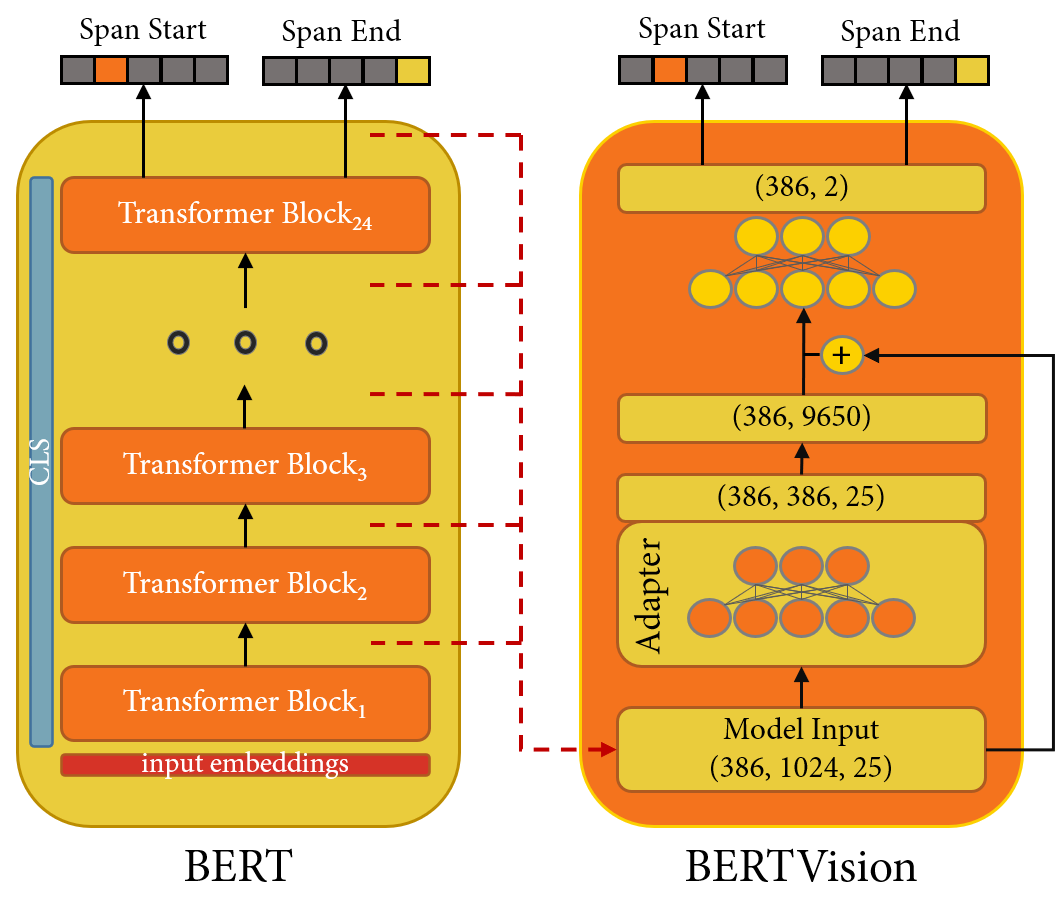
\includegraphics[width=7.5cm]{images/BERTVision_QA_Model.png}}
\end{figure*}
	
	\section{Methods}
\label{sec:methods}

This section introduces our baseline BERT model, and custom models trained on BERT embeddings. We also describe how we use the SQuAD 2.0 question-answering dataset for both span annotation and classification.

\subsection{Modeling approach}

Our custom models use the BERT activations from each encoder layer as input data. For a single SQuAD 2.0 example, our data point has a shape of (X,1024, 25), where $X=386$ for span annotation, and 1 for classification (see appendix [\ref{sec:appendix}] for details). We term this representation of the data as \textit{“embeddings.”}

\subsection{Learned and average pooling}

We implemented the pooling method described in \cite{tenney-etal-2019-bert}, which contracts the last dimension from 25 to 1 through a learned linear combination of each layer. We call this approach learned pooling (LP). We also evaluate the pooling approach reported in \cite{ma2019universal}, average pooling (AP), where each encoder layer is given equal weights. 

\subsection{Adapter compression}

We use the term “compression” to refer to methods that reduce the 1024 dimension of the BERT embeddings. The method proposed in \cite{DBLP:journals/corr/abs-1902-00751} is termed \textit{“adapter”}, which is an auto-encoder type architecture wherein the embeddings are first projected into a lower dimension using a fully-connected layer. For our purposes, the adapter serves as a bridge between BERT embeddings and downstream layers. The architecture in Houlsby et. al. can only handle 3D tensors (including batch), because each adapter handles data from a single transformer layer. Since we work with the activations from multiple layers at once, we need to be able to handle 4D tensors. To do this, our adapter implementation can treat each transformer layer as independent, learning separate compression weights for each layer. Alternatively, we can also employ weight-sharing, so that the compression for each encoder layer follows the same set of transformations.

\subsection{Custom CNN's}

We also implemented various novel CNN architectures, as well as modified existing models such as Inception and Xception \citep{DBLP:journals/corr/SzegedyLJSRAEVR14, DBLP:journals/corr/Chollet16a}. For span annotation, the key is that the CNN models must preserve the text length dimension of 386 (see appendix [\ref{sec:appendix}] for rationale). To view a notebook of all models we tried and their summaries, see: \href{https://github.com/cbenge509/BERTVision}{BERT Vision GitHub repo}.

\subsection{Fine-tuning BERT}

For all experiments, we use the $BERT_{LARGE}$ uncased implementation from \href{https://huggingface.co/}{Hugging Face}. To establish a baseline for our QA tasks, we fine-tuned BERT for 6 epochs with a setup similar to that described in \cite{Devlin2019}. For QA span annotation, questions that do not have answers have the start and end span positions assigned at the CLS token (position 0). We used the Adam optimizer with an initial learning rate of 1e-5. Due to hardware constraints, we use batch size of 8 rather than 48. At inference time, the most likely complete span is predicted based on the maximum softmax probability of the start- and end-span position. The setup is identical in classification, except that we used the pooled CLS token rather than the sequence outputs.
%\begin{equation} \label{eq1}
%Y_{\left(S,E\right)} = \left(\underset{start}{\arg\max} ,\; \underset{end}{\arg\max}\right)
%\end{equation}

\subsection{Ensembling} 

We evaluated multiple ensemble approaches for span annotation. The most successful method presented in this paper takes the element-wise max of the softmax probabilities output by each model. This occurs independently for the start-span position and end-span position. The most likely complete span is then determined by the product of the generated start \& end span vectors.
\begin{equation} \label{eq2}
\begin{aligned}
\text{Let Z be all model softmax probabilities}, \\
K = 386,\;\text{and}\;N = len(Z) \\
\arg\max\left(\prod_{i=1}^{K}{\prod_{j=1}^{N}{Z_{j,i}}}\right)
\end{aligned}
\end{equation}

\subsection{Data processing and evaluation}

We use SQuAD 2.0 for our QA dataset. Standard Exact Match (EM) and F1-score (F1) are used for evaluation as outlined in \cite{DBLP:journals/corr/abs-1806-03822}. For classification, EM is equivalent to accuracy as we are predicting a single binary outcome. For our BERT models, we restrict the maximum token length to 386 (See appendix [\ref{sec:appendix}] for rationale). Question-context pairs that exceed this maximum sequence are split into multiple segments (as many as needed) with an overlap between each segment of 128 tokens. For the splits that do not contain the answer, the labels for that split are set to “no answer”. At inference time, we take the argmax of the span probabilities predicted by each split as the final prediction for the example.
%\begin{equation} \label{eq3}
%EM = \begin{cases} \frac{1}{N}\sum_{i=1}^{N}{\left(\bar{s_i} = s_i,\;\bar{e_i} = e_i\right)} &\mbox{\small if QA} \\
%	\frac{1}{N}\sum_{i=1}^{N}{\left(\bar{s_i} = s_i\right)} &\mbox{\small else}
%	\end{cases} 
%\end{equation}
	\section{Results}

\subsection{BERT Fine-Tuning Partial \& Full Epochs}

In order to establish a baseline performance, we fine-tuned BERT for up to 6 epochs with results shown in Figure [\ref{fig:QnABertPerformance}]. We measure performance for every 10th of a fractional epoch between 0 and 1 epochs, as well as full epochs up to 6. We observed that performanced peaked at 2 epochs, achieving an Exact Match (EM) of 0.747, and an F1 score of 0.792. Between 0 and 1 epochs, performance consistently increased both in terms of EM and F1. For comparison with other published works, see Appendix. \\

In order to select where to extract our hidden state activations, we chose 2 time points to balance training time and model performance. The first is a full training epoch. On our GPU, fine-tuning for 1 epoch is expensive and takes around 5 hours, but performance is already relatively decent compared to peak performance at 2 epochs. This time point gives us high quality embeddings for model development. The second time point is 3/10 of an epoch, which takes about 1.5hr to fine-tune. While cheaper, at this time point, the model has yet to achieve the large jump in performance observed between 3/10 and 4/10 of an epoch. This provides us an opportunity for improvement using our models. 

\begin{figure}[ht]
	\centering
	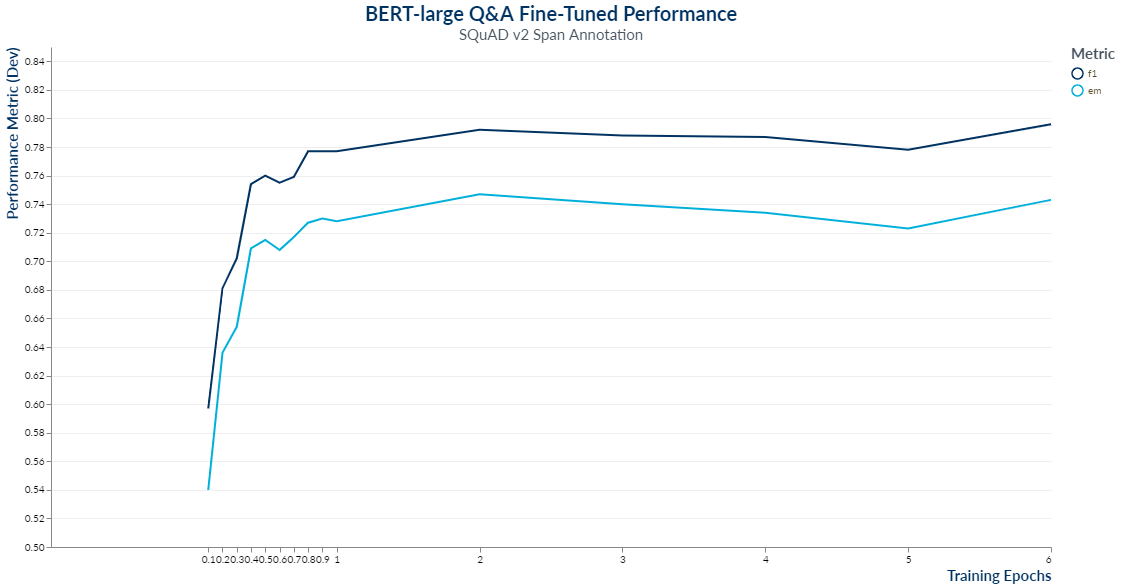
\includegraphics[width=75mm]{images/QnA_BERT_Training_Performance_plot.png}
	\caption{\label{fig:QnABertPerformance}QnA Performance, BERT SQuAD 2.0}
\end{figure}

\subsection{Models trained at 3/10 epoch BERT embeddings}

Using the embeddings at 3/10 of epoch, we explored over 20 parameter-efficient models using a combination of CNNs, pooling and compression techniques. Table [?] shows the performance of our most promising models, and results of all models are in the Appendix. \\

First, we compared two pooling strategies. Our LP (learned pooling) model is identical to the pooling model outlined in Tenney et. al. [?], where weights for combining each encoder layer is learned. The AP (average pooling) model proposed by Ma et. al. [?] on the other hand weights each encoder layer equally. We found that an LP model achieved similar performance as BERT itself, while average pooling significantly decreased performance. An analysis of the learned weights suggests that a non-uniform distribution of pooling weights is optimal, with the distribution slightly favoring later layers of BERT compared to earlier layers (see Appendix). \\

Next, we evaluated the possibility of using adapters modified from Houlsby et. al (see Methods). We found that our modified adapters of all flavors improved model performance compared to baseline BERT. Our best model uses an adapter of size of 386 with weight sharing enabled for each encoder layer, achieving an EM of 0.699 and F1 of 0.740. A skip connection between the final encoder layer and our model’s penultimate hidden layer is also included (see Figure [?]). Without weight-sharing, the number of parameters increases by about 24x, and model performance slightly decreases. While Houlsby et. al. found that an adapter size of 64 provides the best F1 score when used in between transformer blocks, for our purposes, a size of 64 performed worse with or without weight-sharing. Our best adapter model significantly beats BERT fine-tuned to the same level of 3/10 of an epoch by about 4 percentage points in both EM and F1, although we failed to reach performance at 1 full epoch. \\

While we extensively explored stacking pooling with adapters and CNNs, we did not find a model which performed better than our best adapter model. For example, Table [\ref{tbl:3_10_Models}] shows a model where we stacked learned pooling with our best adapter model and abbreviated Xception network. The number of parameters increased by 16x, but performance was no better than pooling alone.

\begin{table}[ht]
	\centering
	\small
	\begin{tabular}{L{3.5cm} C{0.6cm} C{0.6cm} C{0.6cm} C{0.6cm}}
		\hline
		\textbf{Model} (\% params of $BERT_{LARGE}$)       & \textbf{EM $\frac{3}{10}e$} & \textbf{F1 $\frac{3}{10}e$} & \textbf{EM $1e$} & \textbf{F1 $1e$}\Tstrut \\
		\hline
		BERT $\frac{3}{10}e\;\left(100\%\right)$           & $0.654$ & $0.702$ & $0.728$ & $0.777$\Tstrut\Bstrut  \\
		BERT $1e\;\left(100\%\right)$ 					   & $0.670$ & $0.712$ & $0.728$ & $0.777$\Tstrut\Bstrut  \\
		learned pooling $\left(0.001\%\right)$             & $0.660$ & $0.703$ & $0.725$ & $0.759$\Tstrut\Bstrut  \\
		average pooling $\left(0.001\%\right)$             & $0.657$ & $0.700$ & $0.736$ & $0.741$\Tstrut\Bstrut  \\
		\hline\hline
		adapter shared 386 skip $\left(0.124\%\right)$     & \boldmath$0.699$ & \boldmath$0.740$ & \boldmath$0.745$ & \boldmath$0.791$\Tstrut\Bstrut  \\
		\hline\hline
		adapter independent 386 $\left(2.957\%\right)$     & $0.676$ & $0.723$ & $0.730$ & $0.778$\Tstrut\Bstrut  \\
		adapter shared 64 $\left(0.021\%\right)$           & $0.680$ & $0.732$ & $0.722$ & $0.761$\Tstrut\Bstrut  \\
		adapter independent 64$\left(0.491\%\right)$         & $0.684$ & $0.716$ & $0.736$ & $0.782$\Tstrut\Bstrut  \\
		pooling adapter 386 \& xception $\left(1.970\%\right)$         & $0.668$ & $0.711$ & $0.699$ & $0.751$\Tstrut\Bstrut  \\
		\hline
	\end{tabular}
	\caption{\label{tbl:3_10_Models}Models at $\frac{3}{10}$ epochs but evaluated at 1 epoch}
\end{table}

\subsection{Best Models on top at 1 epoch}

Using the embeddings at 1 epoch of fine-tuning, we trained the same set of 20 models as at 3/10 of an epoch of fine-tuning (see the Appendix for a full set of results). In most cases, we found that our models outperformed BERT at 1 epoch of fine-tuning. One exception is our adapter 386 model with independent weights, which suffered about 1 percentage point drop. Table [\ref{dev_set_performance}] shows that adapter models of size 64, with or without weight-sharing, both beat BERT, but the best model found is almost identical to that found at 3/10 of an epoch utilizing an adapter size of 386. The only exception that a skip connection is not needed in this case. This model’s performance is also competitive with maximum performance achieved with BERT fine-tuning, with a slightly improved EM (0.749 vs 0.747) and a slightly decreased F1 (0.790 vs 0.792). This result shows that we are able to reduce BERT fine-tuning by 1 epoch and still achieve similar performance with a model of only about 0.124\% of the number of BERT parameters. 

\begin{table}[ht]
	\centering
	\small
	\begin{tabular}{L{2.8cm} L{1.8cm} C{0.6cm} C{0.6cm}}
		\hline
		\textbf{Model} & \textbf{\% params of} $BERT_{LARGE}$ & \textbf{EM} & \textbf{F1}\Tstrut \\
		\hline
		BERT $1e$ & 100\% 						 & $0.728$ & $0.777$ \\
		BERT $2e$ (\textit{best}) & 100\%		 & $0.747$ & $0.792$ \\
		adapter shared 386 & 0.124\% 			 & $0.749$ & $0.790$ \\
		\hline\hline
		adapter independent 386 & 2.957\% 		 & \boldmath$0.716$ & \boldmath$0.767$ \\
		\hline\hline
		adapter shared 64 & 0.021\% 			 & $0.739$ & $0.785$ \\
		adapter independent 64 & 0.491\% 		 & $0.736$ & $0.784$ \\
		tenney adapter 386 \& xception & 1.970\% & $0.741$ & $0.786$ \\
		\hline
	\end{tabular}
	\caption{\label{tbl:dev_set_performance}Dev set performance}
\end{table}

\subsection{Performance of models trained at 3/10 epoch on higher quality embeddings}

We wanted to better understand why models trained on embeddings derived at 1 epoch of fine-tuning performed better than models trained on embeddings derived at 3/10 of an epoch. In order to do this, we took all of our models trained on the 3/10 embeddings, and evaluated their performance on the dev set with embeddings derived at 1 epoch. To our surprise, all models experienced a significant jump in performance compared to evaluation at embeddings derived at 3/10 of an epoch. Figure [?] shows a comparison of these results on our top models, and Appendix S[?] contains data for all models.  \\

For example, our best model trained at 3/10 of an epoch achieved a performance of 0.745 EM and 0.791 F1 when evaluated on embeddings from 1 epoch. This is a significant boost compared to evaluating the exact same model on embeddings derived from 3/10 of an epoch (0.699 EM and 0.740EM). This model performs similarly to our best model trained on 1 epoch embeddings, and by a transitive relation, also performs similarly to maximum BERT performance at 2 epochs. We consider this a significant achievement for a model that has only seen data from 3/10 of an epoch of fine-tuning. \\

Our result suggests that models trained at 3/10 of an epoch are learning transformations that are transferable even as BERT is further fine-tuned. This implies that BERT is maintaining some level of constancy in the structure of its internal representations. Practically, this means that our models can be trained in parallel with BERT fine-tuning. As BERT learns better internal representations of the data, models trained on earlier representations can leverage this improvement and achieve better performance on the task on hand. \\

\subsection{Training with less data}

The previous sections show that our models perform well compared to BERT when trained on the full dataset. However, since supervised data can be difficult to obtain for certain tasks, we wanted to explore whether our models can perform well with significantly less data. In addition in our case, since embeddings can be expensive to calculate and store, reducing training data also helps with our data management issue (see Methods). To answer this question, we trained our best models (for both 3/10 epoch and 1 epoch embeddings) on varying amounts of data, ranging from 0\% to 100\% of the dataset at step sizes of 10\%. All models were trained for 1 epoch, the same as using the full dataset. Here, 0\% represents randomized weights with no training. For the model at 3/10 of an epoch, we measured its dev set performance on both the 3/10 epoch embeddings and 1 epoch embeddings.  \\

Figure [\ref{fig:1_epoch_embeddings__adapter_386_with_skip}] shows the results. In all cases, we rapidly approach strong performance early on, beating BERT at around 30\% of the data. Even at 10\% of the data, we are only about 3 percentage points in terms of EM, and 2 from F1, from maximum peak performance. This shows that we can in fact achieve strong performance even when using training less. 

\begin{figure}[ht]
	\centering
	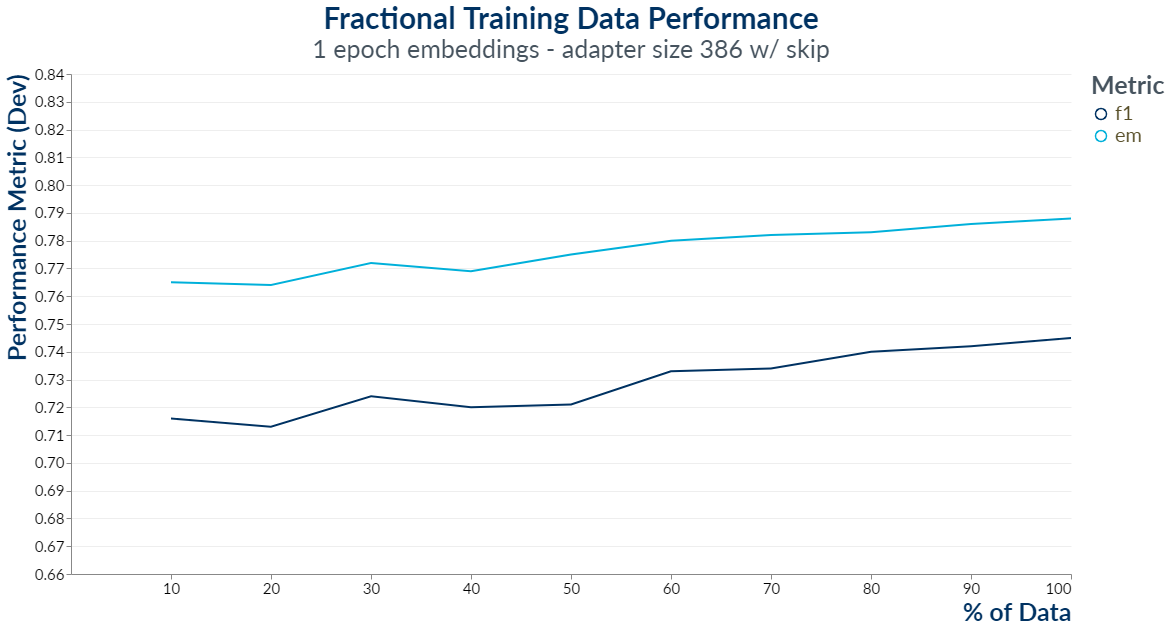
\includegraphics[width=75mm]{images/1_Epoch_Embeddings__Adapter_386_with_Skip.png}
	\caption{\label{fig:1_epoch_embeddings__adapter_386_with_skip}1 epoch embeddings - adapter 386 w/ skip}
\end{figure}

\begin{table}[ht]
	\centering
	\small
	\begin{tabular}{L{0.8cm} C{0.90cm} C{0.90cm} C{1.5cm} C{1.5cm}}
		\hline\Bstrut
		\textbf{\% data} & \textbf{EM} & \textbf{F1} & \textbf{EM \boldmath$1e$ embeddings} & \textbf{F1 \boldmath$1e$ embeddings}  \\
		\hline\Tstrut\Bstrut
		10\%  & $0.633$ & $0.692$ & $0.712$ & $0.768$ \\[.1cm]
		20\%  & $0.633$ & $0.690$ & $0.714$ & $0.767$ \\[.1cm]
		30\%  & $0.660$ & $0.711$ & $0.735$ & $0.782$ \\[.1cm]
		40\%  & $0.663$ & $0.695$ & $0.737$ & $0.775$ \\[.1cm]
		50\%  & $0.673$ & $0.712$ & $0.741$ & $0.783$ \\[.1cm]
		60\%  & $0.681$ & $0.719$ & $0.733$ & $0.772$ \\[.1cm]
		70\%  & $0.683$ & $0.729$ & $0.731$ & $0.779$ \\[.1cm]
		80\%  & $0.686$ & $0.724$ & $0.741$ & \boldmath$0.785$ \\[.1cm]
		90\%  & $0.687$ & $0.734$ & $0.733$ & $0.783$ \\[.1cm]
		100\% & \boldmath$0.689$ & \boldmath$0.733$ & \boldmath$0.736$ & $0.783$ \\[.1cm]
		\hline
	\end{tabular}
	\caption{\label{tbl:3_10_embeddings__adpater_386}$\frac{3}{10}$ Epochs embeddings - adapter 386}
\end{table}



	\section{Model analysis}

\subsection{Question types}

Model performance on SQuAD 2.0 can be categorized based on whether the question-context pair has an answer (Has Answer versus No Answer). The dev set is very balanced in this sense as it contains 5,928 ($\sim$49.93\%) pairs with answers and 5,945 ($\sim$50.07\%) pairs without answers. Figure [\ref{fig:qa_correct_answers_by_model_and_type}] shows the fraction of questions of each type that BERT and our best-performing models correctly answers. As BERT is fine-tuned, the number of correctly answered questions in both categories increases, but questions with “No Answer” increases more rapidly. Our best models answer more “No Answer” questions correctly than BERT, but underperform BERT in terms of “Has Answer” questions.

To investigate further, we looked at our 3/10 epoch model’s incorrect predictions on “Has Answer” questions, and found that a large percentage, $\sim$65\%, were predicted as having no answer (rather than with the wrong answer). These results suggest that our models may be more liberal than BERT at predicting “no answer”.

\begin{figure}[ht]
	\centering
	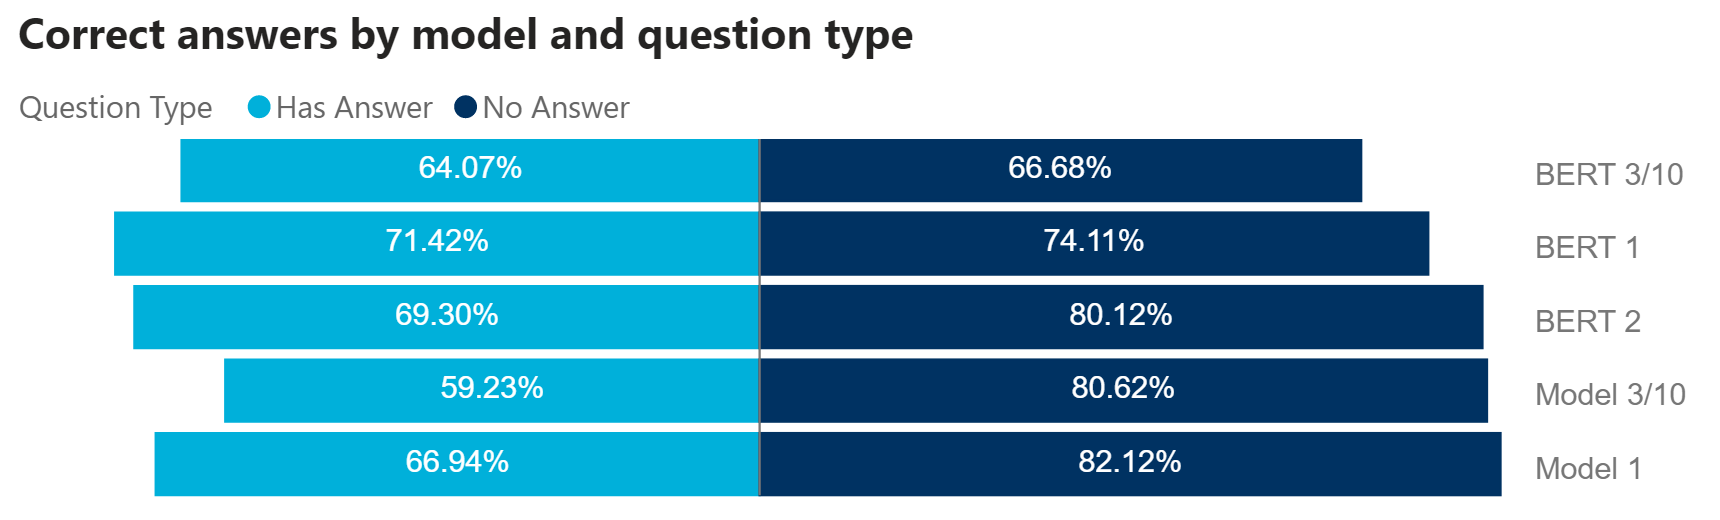
\includegraphics[width=7.5cm]{images/QA_Correct_Answers_by_Question_Type.png}
	\caption{\label{fig:qa_correct_answers_by_model_and_type}Correctly answer percentages by model}
\end{figure}

\subsection{Second most likely answer}

For questions where our 3/10 epoch model’s most likely answer was incorrect, we considered the second most likely answer predicted by the model. We found that the second most likely answer is correct 44\% of the time when the most likely answer is incorrect. We also note 47\% of these were also “Has Answer” questions, which is a more balanced distribution compared to the most likely answer (where only 42\% of correctly answered questions have an answer). This suggests that even though our model at 3/10 is liberal at predicting no answer, its second most likely answer is quite frequently correct and less biased. 

\subsection{Context Length}

The previous section shows that our models are better at recognizing questions with no answers compared to BERT. Here, we look at which models perform better on longer sequences. At 3/10 of an epoch of fine-tuning, BERT and our models performed similarly (BERT average length: 165.86, our model average length: 164.50). However, we believe this is because both models answered correctly many of the same questions. When looking at questions that were uniquely answered correctly by each model, a clear difference emerges: the average sequence length for BERT is longer (BERT: 175.30, our model: 161.68). This suggests that our models are better at answering questions with shorter contexts than BERT. The same trend holds at 1 epoch of fine-tuning.

\subsection{Do 2 epochs perform even better?}
	
Our previous results show that models built on BERT embeddings at 1 epoch achieves maximal BERT performance at 2 epochs. Here, we investigate if we can further improve performance by training directly on embeddings derived at 2 epochs. While this approach does not reduce BERT fine-tuning time, it does provide a way to investigate whether our approach can achieve even better performance with longer fine-tuning. 
	
Table [\ref{tbl:bc_bert_fine_tuning}] shows the results. As expected, the 2-epoch models outperform the same models trained on 1-epoch embeddings. Since ensembling improved performance at 1 epoch, we applied the same approach to the models at 2 epochs. Surprisingly, the 2 epoch ensemble does not outperform the 1 epoch ensemble in terms of either EM (0.749 vs 0.756) or F1 (0.795 vs 0.798). This suggests that additional fine-tuning does not guarantee better performance. Our 1-epoch models, in addition with ensembling, not only saves on BERT fine-tuning time, but also achieves the best possible performance, suggesting a total lack of need for fine-tuning beyond 1 epoch.

\begin{table}[ht]
	\centering
	\small
	\begin{tabular}{L{4.2cm}|C{0.9cm} C{0.9cm}}
		\toprule
		\textbf{Model} & \multicolumn{2}{c}{\textbf{SQuAD2.0}}\\
		& \textbf{EM} & \textbf{F1}\\
		\midrule
		BERT $2e$ (\textit{best}) 		& $0.747$ & $0.792$ \\
		Best model $1e$ 				& $0.753$ & $0.797$ \\
		\textbf{Best model} \boldmath$\frac{3}{10}e$ & \boldmath$0.749$ & \boldmath$0.795$ \\
		ensemble BERT $2e$ + best $1e$	& $0.751$ & $0.796$ \\
		\bottomrule
	\end{tabular}
	\caption{\label{tbl:bc_bert_fine_tuning}2 epochs embeddings evaluation results}
\end{table}

	\section{Conclusion and future work}

In this paper, we propose a parameter-efficient approach that achieves maximal BERT performance for QA span annotation and greatly reduces fine-tuning time required for BERT. Our models are trained on BERT hidden state activations (embeddings), and consistently outperform BERT at the same level of fine-tuning. By using an ensemble of our model with BERT’s predictions, we further surpass BERT performance, reducing the need for fine-tuning by 1 epoch. We achieved similarly promising results for QA classification, which suggests that this approach works well with both the full sequence BERT embeddings and with the CLS token embedding. Future work might look at reducing fine-tuning even further, by focusing on modeling, or alternative approaches for combining BERT embeddings. Better data caching strategies could also help the practical application of this method in production, as data loading from disk can be slow for generic hardware. While this work focused on SQuAD 2.0, further work can also evaluate this method on other NLP tasks, such as GLUE. Success here would demonstrate the ability of the method to generalize beyond QA, including for advanced inference tasks, such as entailment and paraphrasing. Overall, we demonstrated as a proof-of-concept that BERT embeddings carries valuable information that can be leveraged for inference, in a way that reduces BERT fine-tuning and exceed BERT performance.

	% ---------------------------------------------------------------------------
	% formatting examples; we will throw this out when paper is done.
	% ---------------------------------------------------------------------------
	%\section{Formatting Instructions}

Manuscripts must be in two-column format.
Exceptions to the two-column format include the title, authors' names and complete addresses, which must be centered at the top of the first page, and any full-width figures or tables (see the guidelines in Section~\ref{ssec:title-authors}).
\textbf{Type single-spaced.}
Start all pages directly under the top margin.
The manuscript should be printed single-sided and its length should not exceed the maximum page limit described in Section~\ref{sec:length}.
Pages should be numbered in the version submitted for review, but \textbf{pages should not be numbered in the camera-ready version}.

\paragraph{\LaTeX-specific details:}
The style files will generate page numbers when {\small\verb|\aclfinalcopy|} is commented out, and remove them otherwise.


\subsection{File Format}
\label{sect:pdf}

For the production of the electronic manuscript you must use Adobe's Portable Document Format (PDF).
Please make sure that your PDF file includes all the necessary fonts (especially tree diagrams, symbols, and fonts with Asian characters).
When you print or create the PDF file, there is usually an option in your printer setup to include none, all or just non-standard fonts.
Please make sure that you select the option of including ALL the fonts.
\textbf{Before sending it, test your PDF by printing it from a computer different from the one where it was created.}
Moreover, some word processors may generate very large PDF files, where each page is rendered as an image.
Such images may reproduce poorly.
In this case, try alternative ways to obtain the PDF.
One way on some systems is to install a driver for a postscript printer, send your document to the printer specifying ``Output to a file'', then convert the file to PDF.

It is of utmost importance to specify the \textbf{A4 format} (21 cm x 29.7 cm) when formatting the paper.
Print-outs of the PDF file on A4 paper should be identical to the hardcopy version.
If you cannot meet the above requirements about the production of your electronic submission, please contact the publication chairs as soon as possible.

\paragraph{\LaTeX-specific details:}
PDF files are usually produced from \LaTeX{} using the \texttt{\small pdflatex} command.
If your version of \LaTeX{} produces Postscript files, \texttt{\small ps2pdf} or \texttt{\small dvipdf} can convert these to PDF.
To ensure A4 format in \LaTeX, use the command {\small\verb|\special{papersize=210mm,297mm}|}
in the \LaTeX{} preamble (below the {\small\verb|\usepackage|} commands) and use \texttt{\small dvipdf} and/or \texttt{\small pdflatex}; or specify \texttt{\small -t a4} when working with \texttt{\small dvips}.

\subsection{Layout}
\label{ssec:layout}

Format manuscripts two columns to a page, in the manner these
instructions are formatted.
The exact dimensions for a page on A4 paper are:

\begin{itemize}
\item Left and right margins: 2.5 cm
\item Top margin: 2.5 cm
\item Bottom margin: 2.5 cm
\item Column width: 7.7 cm
\item Column height: 24.7 cm
\item Gap between columns: 0.6 cm
\end{itemize}

\noindent Papers should not be submitted on any other paper size.
If you cannot meet the above requirements about the production of your electronic submission, please contact the publication chairs above as soon as possible.

\subsection{Fonts}

For reasons of uniformity, Adobe's \textbf{Times Roman} font should be used.
If Times Roman is unavailable, you may use Times New Roman or \textbf{Computer Modern Roman}.

Table~\ref{font-table} specifies what font sizes and styles must be used for each type of text in the manuscript.

\begin{table}
\centering
\begin{tabular}{lrl}
\hline \textbf{Type of Text} & \textbf{Font Size} & \textbf{Style} \\ \hline
paper title & 15 pt & bold \\
author names & 12 pt & bold \\
author affiliation & 12 pt & \\
the word ``Abstract'' & 12 pt & bold \\
section titles & 12 pt & bold \\
subsection titles & 11 pt & bold \\
document text & 11 pt  &\\
captions & 10 pt & \\
abstract text & 10 pt & \\
bibliography & 10 pt & \\
footnotes & 9 pt & \\
\hline
\end{tabular}
\caption{\label{font-table} Font guide. }
\end{table}

\paragraph{\LaTeX-specific details:}
To use Times Roman in \LaTeX2e{}, put the following in the preamble:
\begin{quote}
\small
\begin{verbatim}
\usepackage{times}
\usepackage{latexsym}
\end{verbatim}
\end{quote}


\subsection{Ruler}
A printed ruler (line numbers in the left and right margins of the article) should be presented in the version submitted for review, so that reviewers may comment on particular lines in the paper without circumlocution.
The presence or absence of the ruler should not change the appearance of any other content on the page.
The camera ready copy should not contain a ruler.

\paragraph{Reviewers:}
note that the ruler measurements may not align well with lines in the paper -- this turns out to be very difficult to do well when the paper contains many figures and equations, and, when done, looks ugly.
In most cases one would expect that the approximate location will be adequate, although you can also use fractional references (\emph{e.g.}, this line ends at mark $295.5$).

\paragraph{\LaTeX-specific details:}
The style files will generate the ruler when {\small\verb|\aclfinalcopy|} is commented out, and remove it otherwise.

\subsection{Title and Authors}
\label{ssec:title-authors}

Center the title, author's name(s) and affiliation(s) across both columns.
Do not use footnotes for affiliations.
Place the title centered at the top of the first page, in a 15-point bold font.
Long titles should be typed on two lines without a blank line intervening.
Put the title 2.5 cm from the top of the page, followed by a blank line, then the author's names(s), and the affiliation on the following line.
Do not use only initials for given names (middle initials are allowed).
Do not format surnames in all capitals (\emph{e.g.}, use ``Mitchell'' not ``MITCHELL'').
Do not format title and section headings in all capitals except for proper names (such as ``BLEU'') that are
conventionally in all capitals.
The affiliation should contain the author's complete address, and if possible, an electronic mail address.

The title, author names and addresses should be completely identical to those entered to the electronical paper submission website in order to maintain the consistency of author information among all publications of the conference.
If they are different, the publication chairs may resolve the difference without consulting with you; so it is in your own interest to double-check that the information is consistent.

Start the body of the first page 7.5 cm from the top of the page.
\textbf{Even in the anonymous version of the paper, you should maintain space for names and addresses so that they will fit in the final (accepted) version.}


\subsection{Abstract}
Use two-column format when you begin the abstract.
Type the abstract at the beginning of the first column.
The width of the abstract text should be smaller than the
width of the columns for the text in the body of the paper by 0.6 cm on each side.
Center the word \textbf{Abstract} in a 12 point bold font above the body of the abstract.
The abstract should be a concise summary of the general thesis and conclusions of the paper.
It should be no longer than 200 words.
The abstract text should be in 10 point font.

\subsection{Text}
Begin typing the main body of the text immediately after the abstract, observing the two-column format as shown in the present document.

Indent 0.4 cm when starting a new paragraph.

\subsection{Sections}

Format section and subsection headings in the style shown on the present document.
Use numbered sections (Arabic numerals) to facilitate cross references.
Number subsections with the section number and the subsection number separated by a dot, in Arabic numerals.

\subsection{Footnotes}
Put footnotes at the bottom of the page and use 9 point font.
They may be numbered or referred to by asterisks or other symbols.\footnote{This is how a footnote should appear.}
Footnotes should be separated from the text by a line.\footnote{Note the line separating the footnotes from the text.}

\subsection{Graphics}

Place figures, tables, and photographs in the paper near where they are first discussed, rather than at the end, if possible.
Wide illustrations may run across both columns.
Color is allowed, but adhere to Section~\ref{ssec:accessibility}'s guidelines on accessibility.

\paragraph{Captions:}
Provide a caption for every illustration; number each one sequentially in the form:
``Figure 1. Caption of the Figure.''
``Table 1. Caption of the Table.''
Type the captions of the figures and tables below the body, using 10 point text.
Captions should be placed below illustrations.
Captions that are one line are centered (see Table~\ref{font-table}).
Captions longer than one line are left-aligned (see Table~\ref{tab:accents}).

\begin{table}
\centering
\begin{tabular}{lc}
\hline
\textbf{Command} & \textbf{Output}\\
\hline
\verb|{\"a}| & {\"a} \\
\verb|{\^e}| & {\^e} \\
\verb|{\`i}| & {\`i} \\ 
\verb|{\.I}| & {\.I} \\ 
\verb|{\o}| & {\o} \\
\verb|{\'u}| & {\'u}  \\ 
\verb|{\aa}| & {\aa}  \\\hline
\end{tabular}
\begin{tabular}{lc}
\hline
\textbf{Command} & \textbf{Output}\\
\hline
\verb|{\c c}| & {\c c} \\ 
\verb|{\u g}| & {\u g} \\ 
\verb|{\l}| & {\l} \\ 
\verb|{\~n}| & {\~n} \\ 
\verb|{\H o}| & {\H o} \\ 
\verb|{\v r}| & {\v r} \\ 
\verb|{\ss}| & {\ss} \\
\hline
\end{tabular}
\caption{Example commands for accented characters, to be used in, \emph{e.g.}, \BibTeX\ names.}\label{tab:accents}
\end{table}

\paragraph{\LaTeX-specific details:}
The style files are compatible with the caption and subcaption packages; do not add optional arguments.
\textbf{Do not override the default caption sizes.}


\subsection{Hyperlinks}
Within-document and external hyperlinks are indicated with Dark Blue text, Color Hex \#000099.

\subsection{Citations}
Citations within the text appear in parentheses as~\citep{Kim2016} or, if the author's name appears in the text itself, as \citet{Kim2016}.
Append lowercase letters to the year in cases of ambiguities.  
Treat double authors as in~\citep{Rajpurkar2016}, but write as in~\citep{Devlin2019} when more than two authors are involved. Collapse multiple citations as in~\citep{Devlin2019,Kim2016}. 

Refrain from using full citations as sentence constituents.
Instead of
\begin{quote}
  ``\citep{Devlin2019} showed that ...''
\end{quote}
write
\begin{quote}
``\citet{Devlin2019} showed that ...''
\end{quote}

\begin{table*}
\centering
\begin{tabular}{lll}
\hline
\textbf{Output} & \textbf{natbib command} & \textbf{Old ACL-style command}\\
\hline
\citep{Devlin2019} & \small\verb|\citep| & \small\verb|\cite| \\
\citealp{Devlin2019} & \small\verb|\citealp| & no equivalent \\
\citet{Devlin2019} & \small\verb|\citet| & \small\verb|\newcite| \\
\citeyearpar{Devlin2019} & \small\verb|\citeyearpar| & \small\verb|\shortcite| \\
\hline
\end{tabular}
\caption{\label{citation-guide}
Citation commands supported by the style file.
The style is based on the natbib package and supports all natbib citation commands.
It also supports commands defined in previous ACL style files for compatibility.
}
\end{table*}

\paragraph{\LaTeX-specific details:}
Table~\ref{citation-guide} shows the syntax supported by the style files.
We encourage you to use the natbib styles.
You can use the command {\small\verb|\citet|} (cite in text) to get ``author (year)'' citations as in \citet{Devlin2019}.
You can use the command {\small\verb|\citep|} (cite in parentheses) to get ``(author, year)'' citations as in \citep{Devlin2019}.
You can use the command {\small\verb|\citealp|} (alternative cite without  parentheses) to get ``author year'' citations (which is useful for  using citations within parentheses, as in \citealp{Devlin2019}).


\subsection{References}
Gather the full set of references together under the heading \textbf{References}; place the section before any Appendices. 
Arrange the references alphabetically by first author, rather than by order of occurrence in the text.

Provide as complete a citation as possible, using a consistent format, such as the one for \emph{Computational Linguistics\/} or the one in the  \emph{Publication Manual of the American 
Psychological Association\/}~\citep{Limaye2019}.
Use full names for authors, not just initials.

Submissions should accurately reference prior and related work, including code and data.
If a piece of prior work appeared in multiple venues, the version that appeared in a refereed, archival venue should be referenced.
If multiple versions of a piece of prior work exist, the one used by the authors should be referenced.
Authors should not rely on automated citation indices to provide accurate references for prior and related work.

The following text cites various types of articles so that the references section of the present document will include them.
\begin{itemize}
\item Example article in journal: \citep{Limaye2019}.
\item Example article in proceedings, with location: \citep{Limaye2019}.
\item Example article in proceedings, without location: \citep{Limaye2019}.
\item Example arxiv paper: \citep{Limaye2019}. 
\end{itemize}


\paragraph{\LaTeX-specific details:}
The \LaTeX{} and Bib\TeX{} style files provided roughly follow the American Psychological Association format.
If your own bib file is named \texttt{\small acl2020.bib}, then placing the following before any appendices in your \LaTeX{}  file will generate the references section for you:
\begin{quote}\small
\verb|\bibliographystyle{acl_natbib}|\\
\verb|\bibliography{acl2020}|
\end{quote}

You can obtain the complete ACL Anthology as a Bib\TeX\ file from \url{https://aclweb.org/anthology/anthology.bib.gz}.
To include both the anthology and your own bib file, use the following instead of the above.
\begin{quote}\small
\verb|\bibliographystyle{acl_natbib}|\\
\verb|\bibliography{anthology,acl2020}|
\end{quote}


\subsection{Digital Object Identifiers}
As part of our work to make ACL materials more widely used and cited outside of our discipline, ACL has registered as a CrossRef member, as a registrant of Digital Object Identifiers (DOIs), the standard for registering permanent URNs for referencing scholarly materials.

All camera-ready references are required to contain the appropriate DOIs (or as a second resort, the hyperlinked ACL Anthology Identifier) to all cited works.
Appropriate records should be found for most materials in the current ACL Anthology at \url{http://aclanthology.info/}.
As examples, we cite \citep{Limaye2019} to show you how papers with a DOI will appear in the bibliography.
We cite \citep{Limaye2019} to show how papers without a DOI but with an ACL Anthology Identifier will appear in the bibliography.

\paragraph{\LaTeX-specific details:}
Please ensure that you use Bib\TeX\ records that contain DOI or URLs for any of the ACL materials that you reference.
If the Bib\TeX{} file contains DOI fields, the paper title in the references section will appear as a hyperlink to the DOI, using the hyperref \LaTeX{} package.


\subsection{Appendices}
Appendices, if any, directly follow the text and the
references (but only in the camera-ready; see Appendix~\ref{sec:appendix}).
Letter them in sequence and provide an informative title:
\textbf{Appendix A. Title of Appendix}.

	% ---------------------------------------------------------------------------

	\section*{Acknowledgments}

We are incredibly thankful for the faculty and instructors of W266 : \textit{Natural Language Processing with Deep Learning} for their guidance, patience, and detailed feedback over the course of this project. In particular, we call out special thanks to Daniel Cer, PhD and Joachim Rahmfeld without whom we would not have escaped the tangled maze of BERT hidden activations in time.

	%\nocite{*}
	\bibliography{references}
	\bibliographystyle{acl_natbib}

	\appendix

\section{Appendices}
\label{sec:appendix}
\small

\subsection{BERT fine-tuning figures}
\label{apdx:BERT_fine_tuning_span_annotation_sec}

BERT$_{large}$ was fine-tuned for both span annotation and classification tasks; below are tables and blots indicating the performance for each task.

\begin{figure}[h]
	\centering
	\begin{subfigure}{0.95\textwidth}%
		\centering
		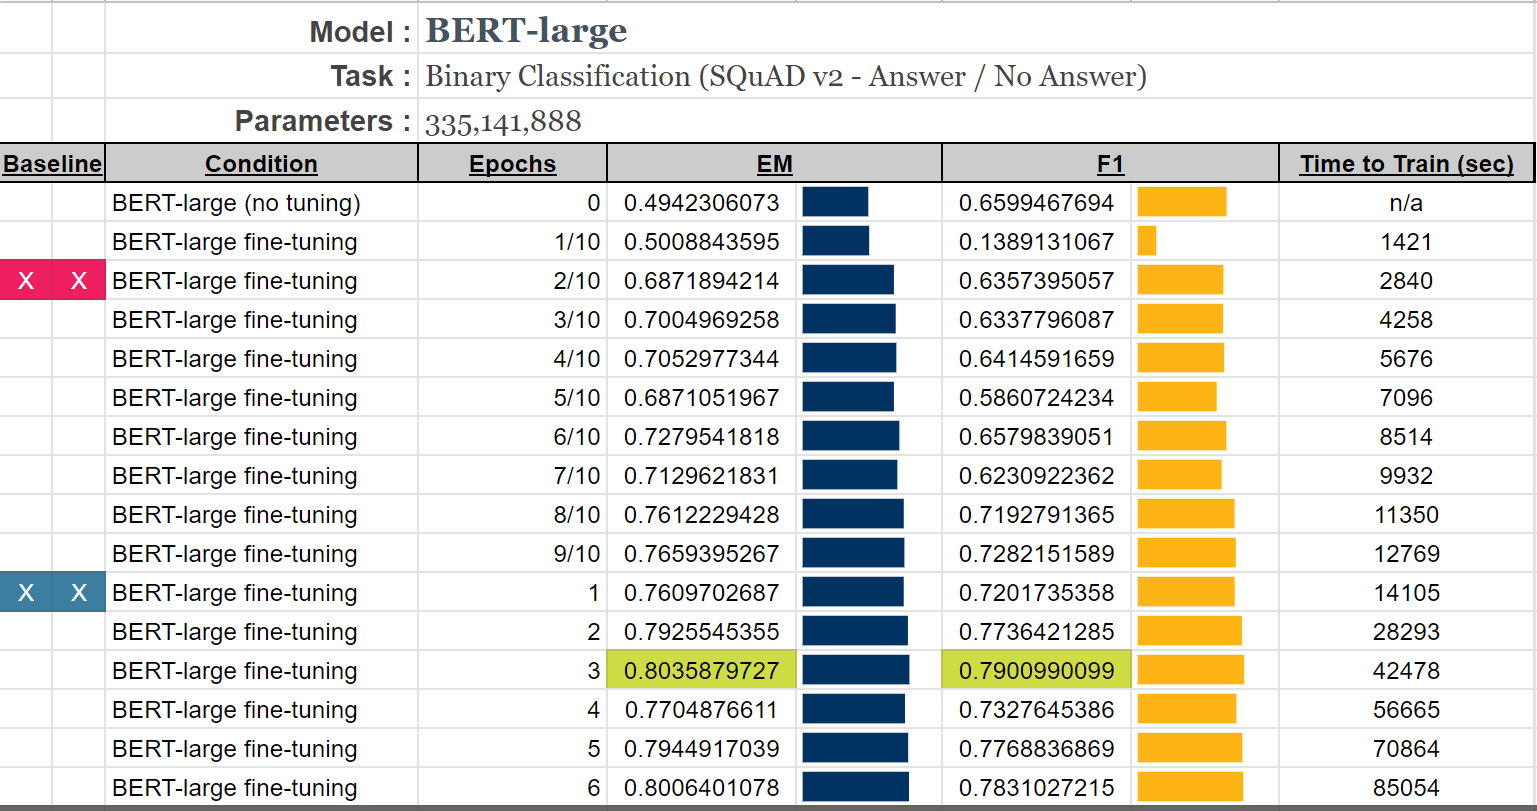
\includegraphics[width=\linewidth]{images/classification/BERT_Large_Training.png}%
		\caption{BERT$_{large}$ fine-tuning table : classification}
	\end{subfigure}%

	\vspace*{8pt}%
	
	\begin{subfigure}{0.96\textwidth}%
		\centering
		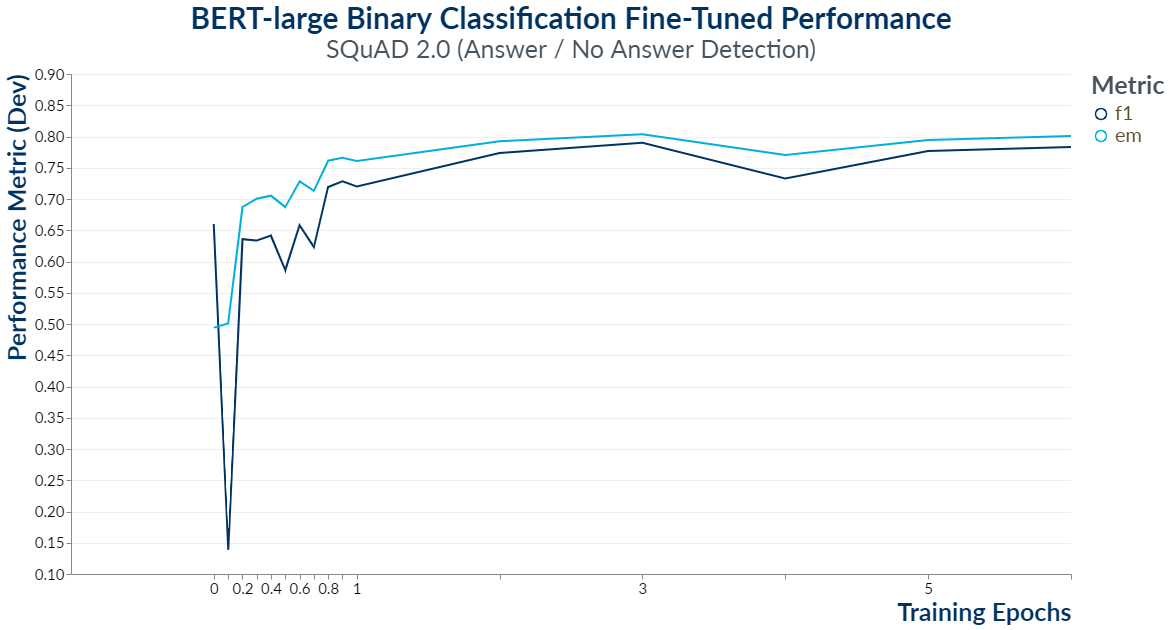
\includegraphics[width=\linewidth]{images/BinaryClassification_BERT_Training_Performance_plot.png}%
		\caption{BERT$_{large}$ fine-tuning plot : classification}
	\end{subfigure}%
	\caption{\label{apdx:BERT_fine_tuning_classification}BERT$_{large}$ fine-tuning for classification}
\end{figure}%

\begin{figure}[!h]
	\centering
	\begin{subfigure}{0.95\textwidth}%
		\centering
		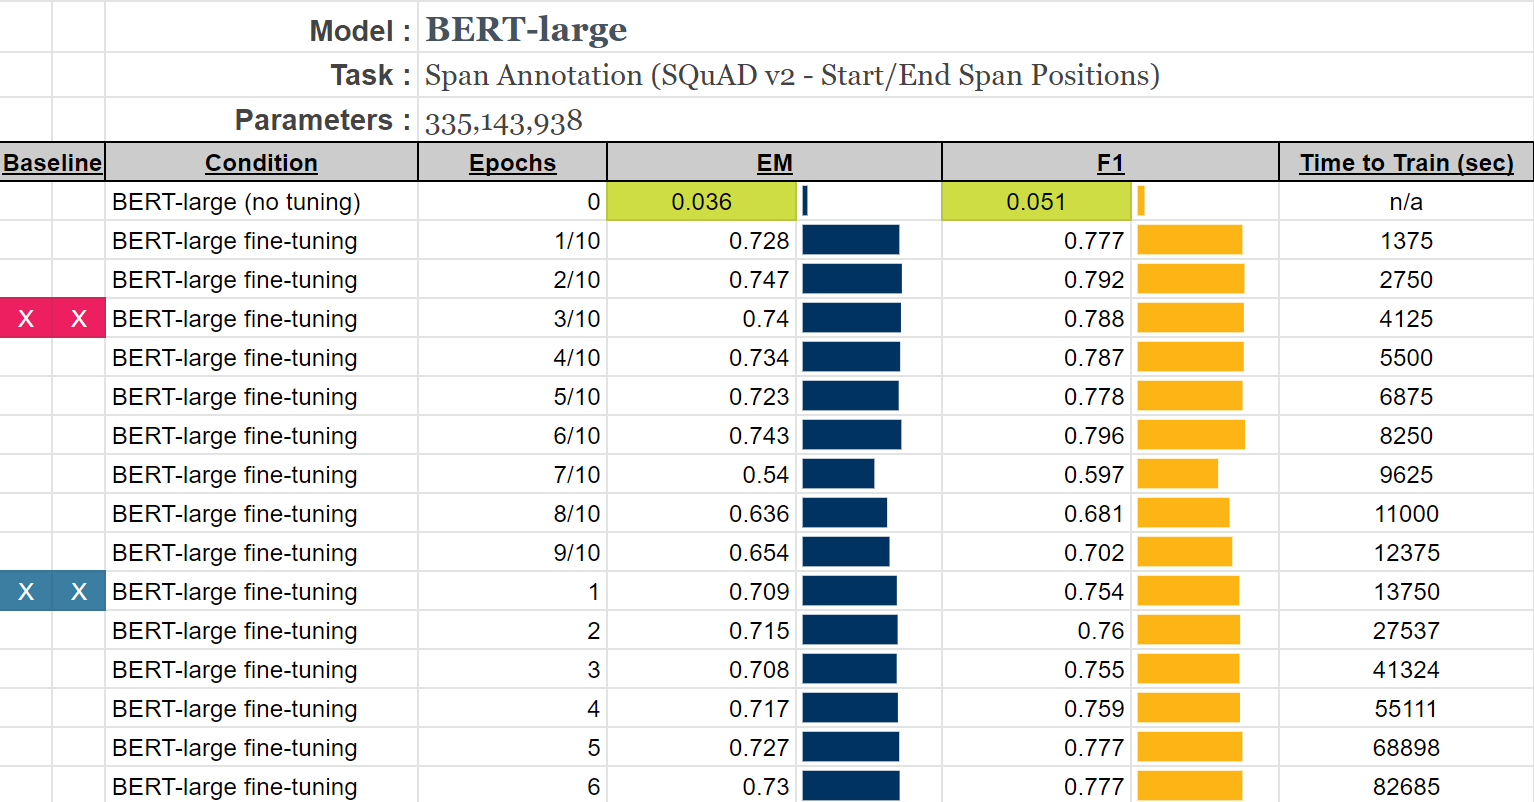
\includegraphics[width=\linewidth]{images/span/BERT_Large_Training.png}%
		\caption{BERT$_{large}$ fine-tuning table : span annotation}
	\end{subfigure}%
	
	\vspace*{8pt}%

	\begin{subfigure}{0.96\textwidth}%
		\centering
		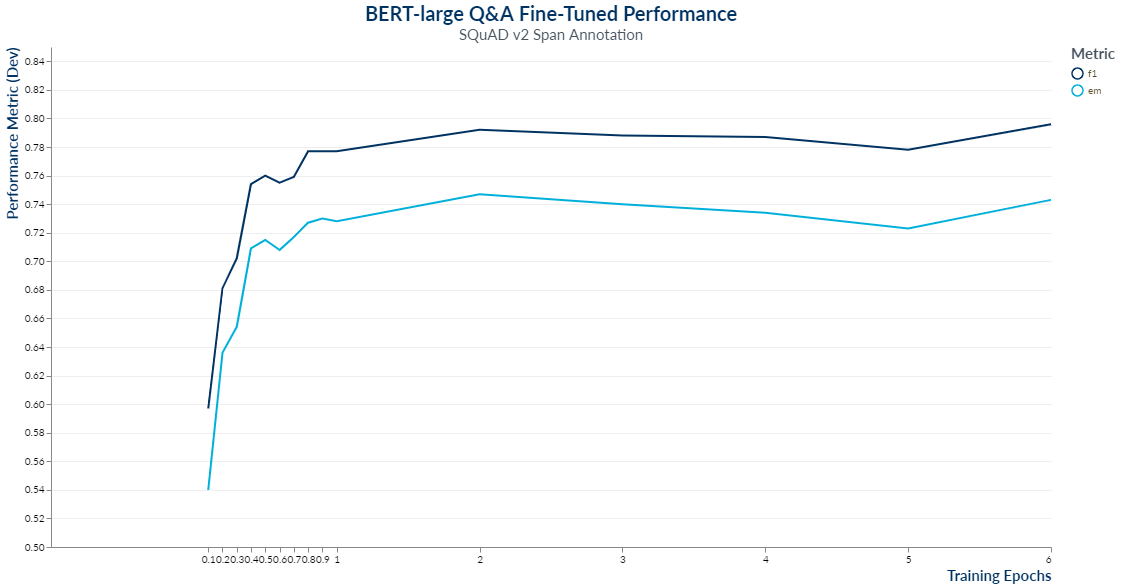
\includegraphics[width=\linewidth]{images/QnA_BERT_Training_Performance_plot.png}%
		\caption{BERT$_{large}$ fine-tuning plot : span annotation}
	\end{subfigure}%
	\caption{\label{apdx:BERT_fine_tuning_span_annotation}BERT$_{large}$ fine-tuning for span annotation}
\end{figure}

\newpage
\subsection{Table of all model results for span annotation}
\label{apdx:span_annotation_all_results}

Models were trained on embeddings derived from 3/10 of an epoch and 1 full epoch.  Performance on evaluation of the dev set is presented below.

\begin{figure}[h]
	\centering
	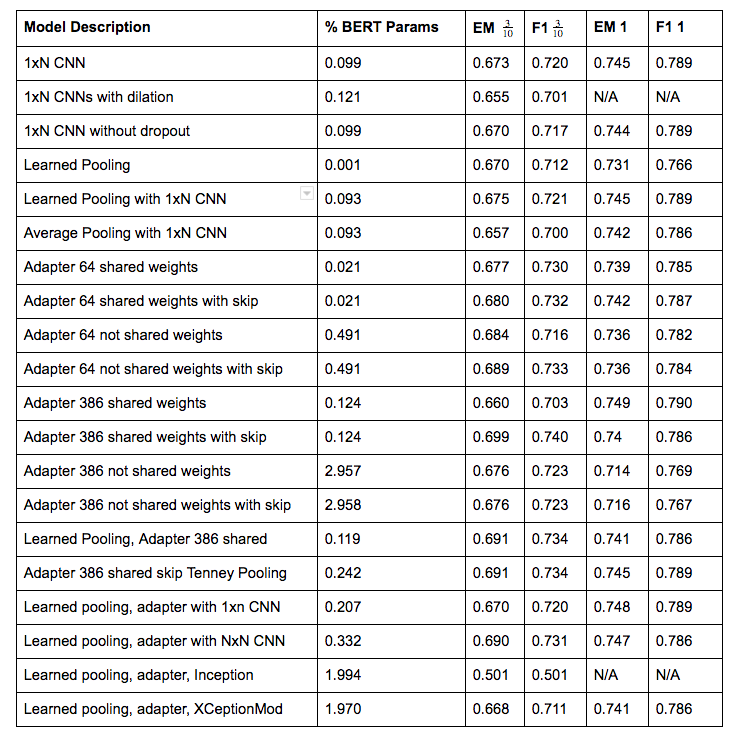
\includegraphics[width=\linewidth]{images/span/Span_Annotation_All_Model_Results.png}%
	\caption{BERT$_{large}$ All model performance : span annotation}
\end{figure}

\subsection{Best model performance for classification task}

The best model evaluated for the classification task was a simple linear model that performed channel contraction using learned weights followed by a simple dense layer connection with no softmax.  As indicated below, this model outperformed BERT$_{large}$ for almost every metric save for F1 on 3 epoch fine-tuned embeddings.

\begin{figure}[h]
	\centering
	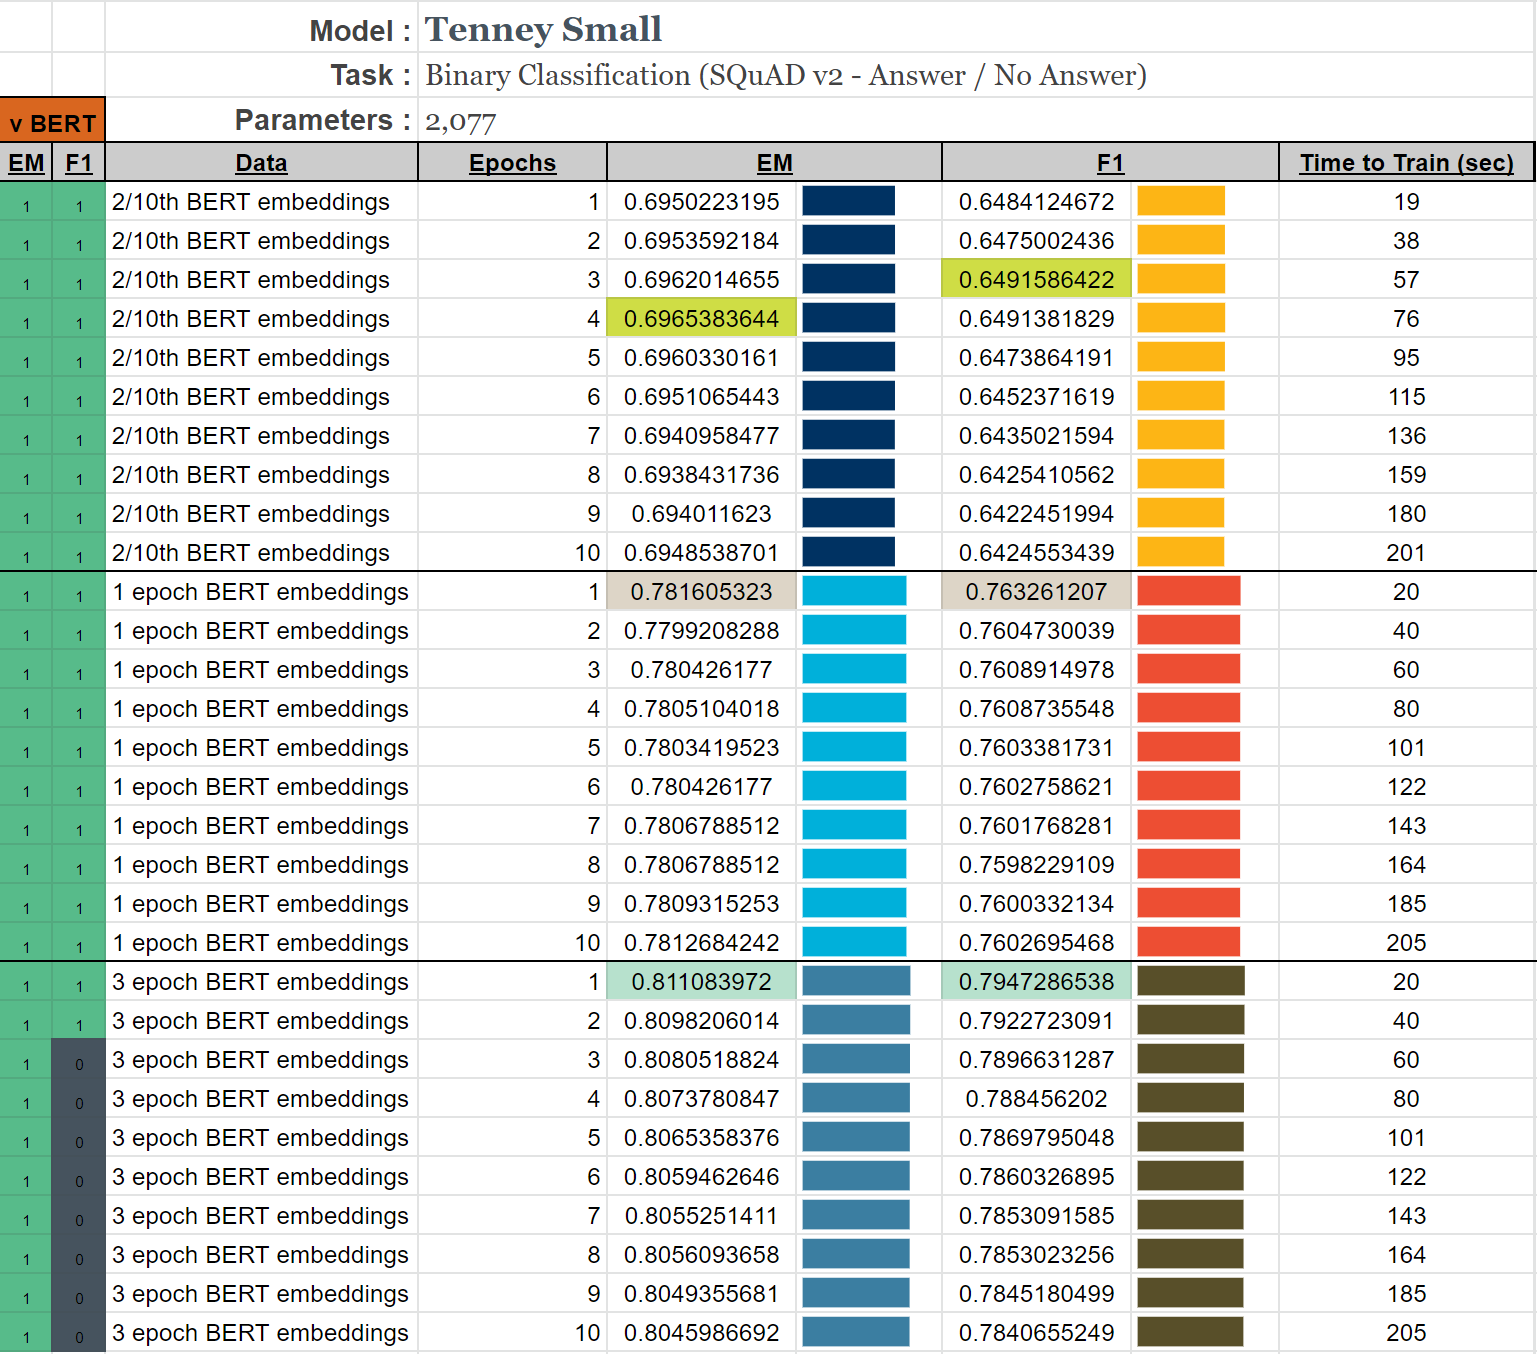
\includegraphics[width=\linewidth]{images/classification/TenneySmall_Training.png}%
	\caption{BERT$_{large}$ Best model performance : classification task}
\end{figure}

\newpage

\begin{figure*}[t]
	\centering
	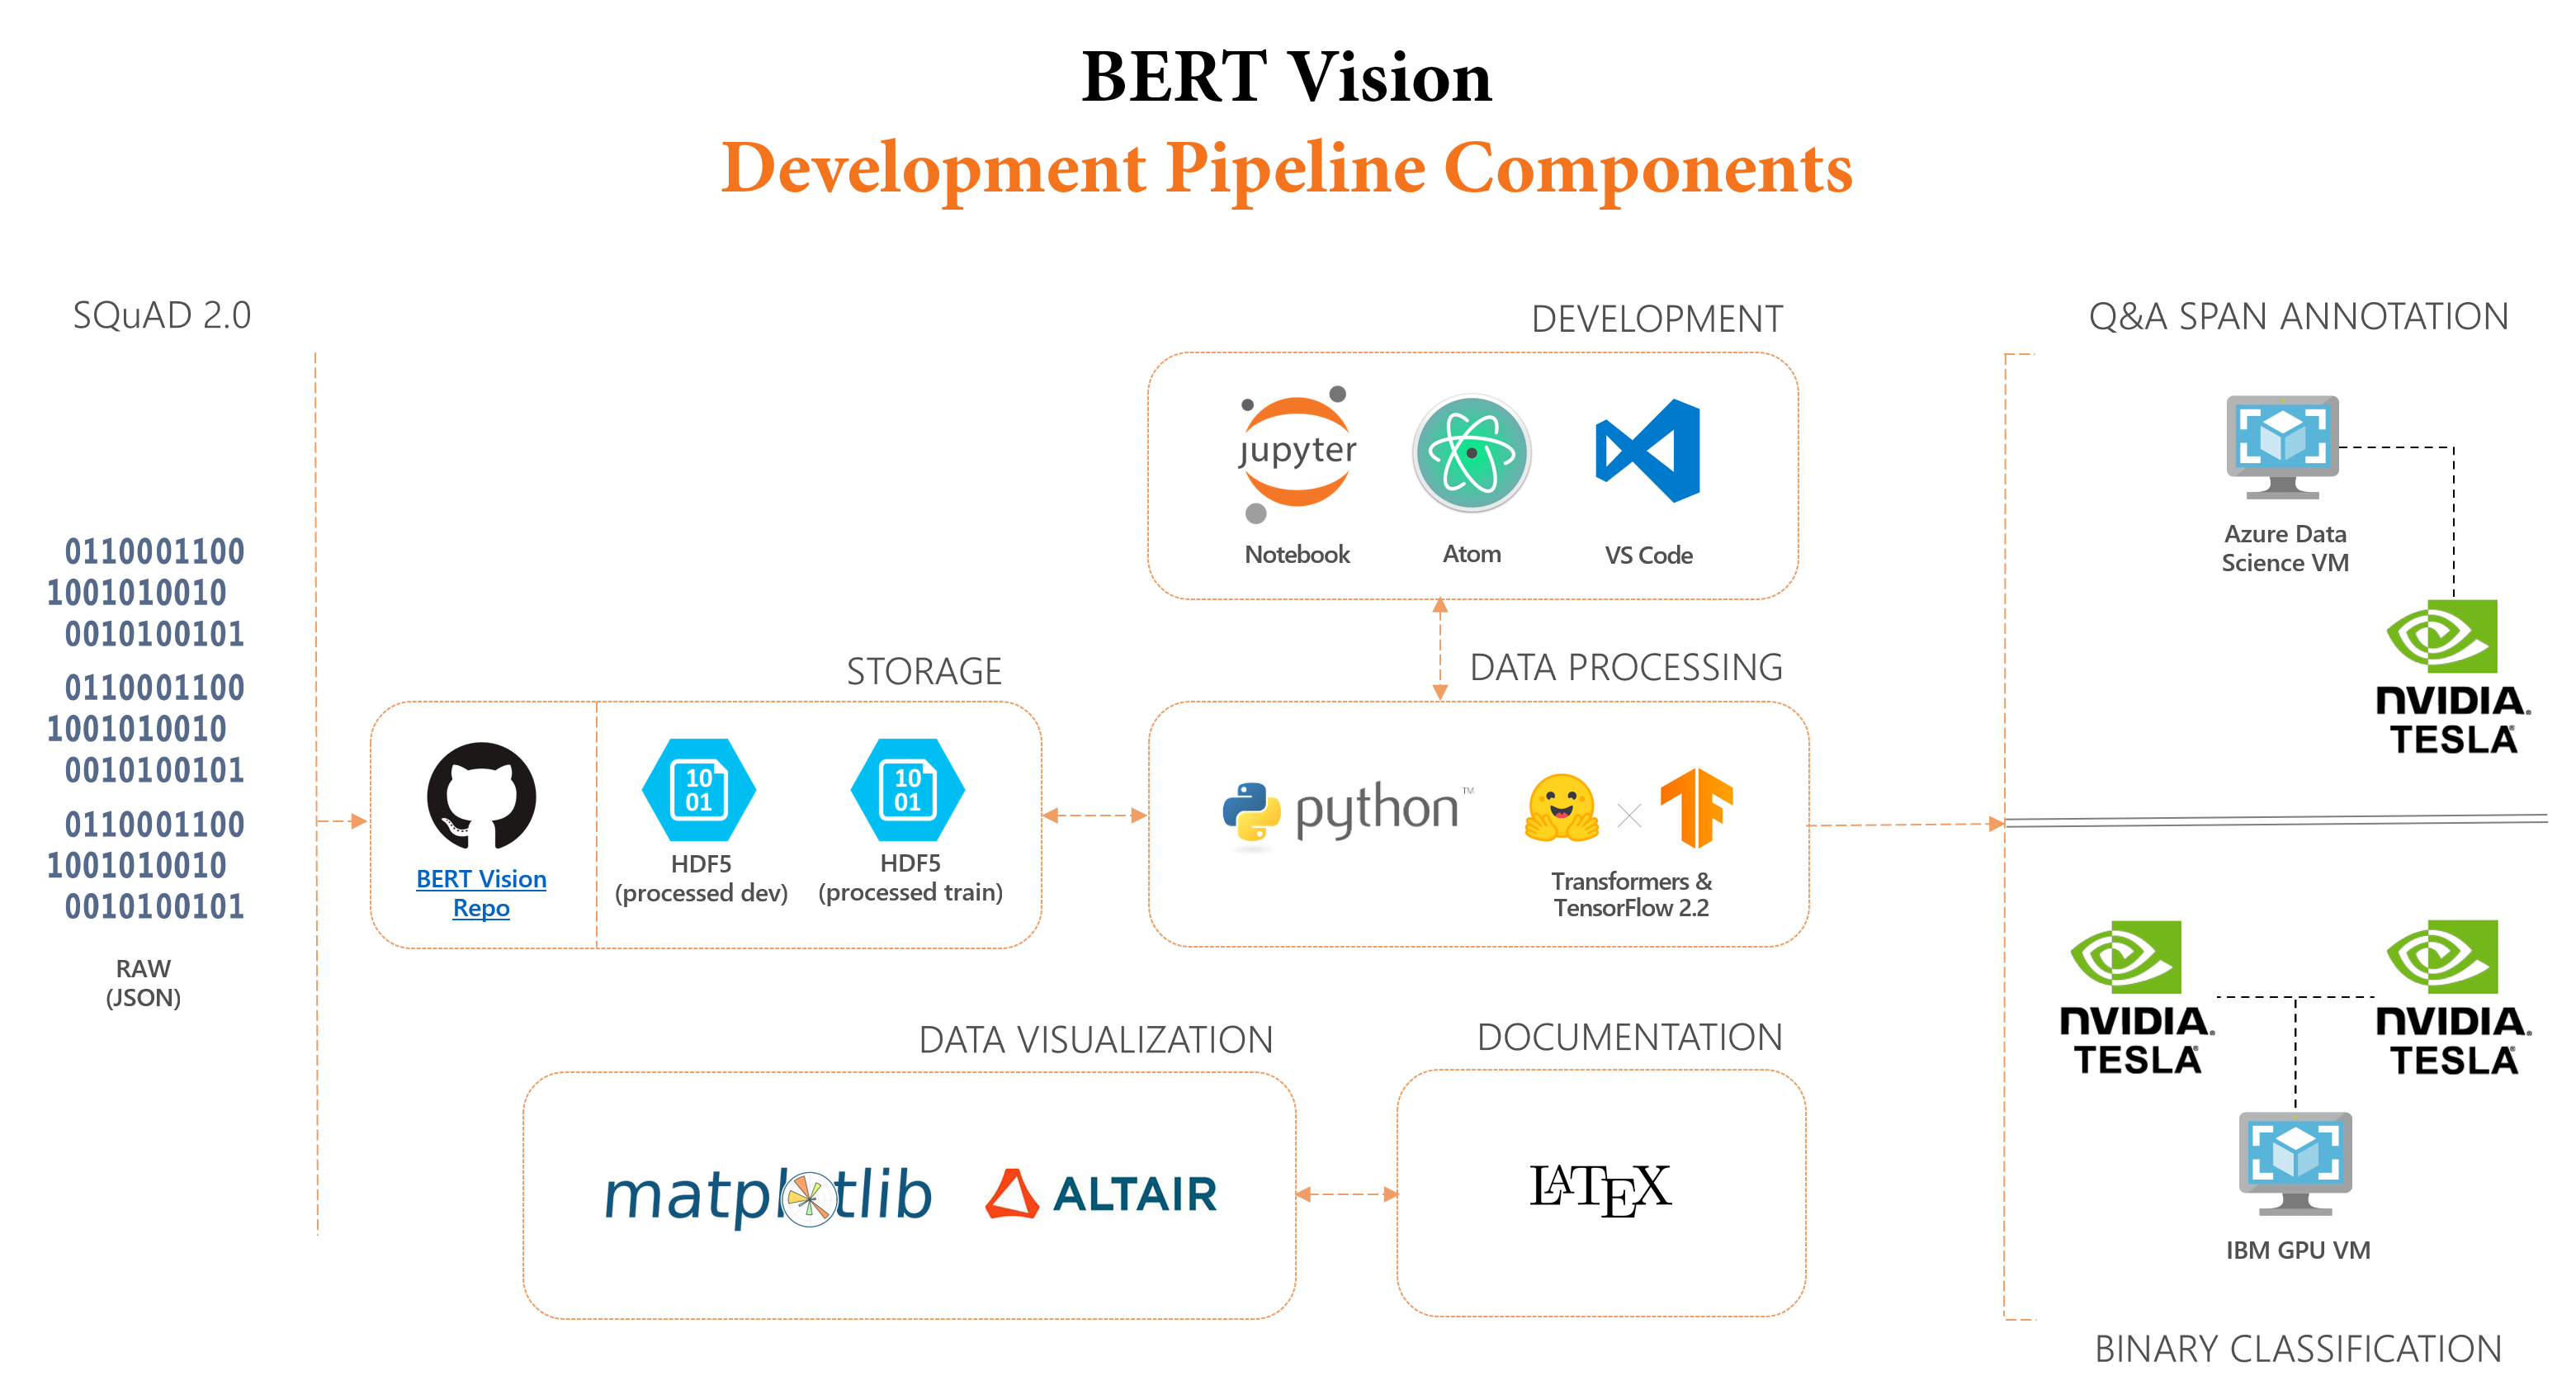
\includegraphics[width=\textwidth]{images/BERTVision_Development_PIpeline.png}%
	\caption{BERTVision development pipeline}
	\label{apdx:bertvision_development_pipeline_graph}
\end{figure*}

\newpage

\subsection{Table of all model results for classification}
\label{apdx:classification_models_trained}

Models were trained on BERT$_{large}$ fine-tuned embeddings derived from 2/10 of an epoch and 1 full epoch. Additionally, the most successful model was trained on 3 epochs fine-tuned embeddings. Performance on evaluation of the dev set is presented below.

\begin{table}[h]
	\centering
	\small
	\begin{tabular}{L{2.9cm}|C{1.5cm} C{0.9cm} C{0.9cm}}
		\toprule
		\textbf{Model} & \textbf{\% Params} & \multicolumn{2}{c}{\textbf{SQuAD2.0}}\\
		& \textbf{BERT}$_{large}$ & \textbf{EM} & \textbf{F1}\\
		\midrule
		adapter pooler tenney 	& 0.119\% & 0.685 & 0.646 \\
		xception abbr 			& 0.079\% & 0.673 & 0.702 \\
		\textbf{xception}		& \textbf{6.181\%} & \textbf{0.707} & \textbf{0.710} \\
		xception abbr cls 		& 0.080\% & 0.672 & 0.564 \\
		adapter pooler avg 		& 0.119\% & 0.691 & 0.624 \\
		tenney small 			& 0.001\% & 0.697 & 0.650 \\
		\bottomrule
	\end{tabular}
	\caption{Models trained on embeddings at $\frac{2}{10}e$}
\end{table}

\begin{table}[h]
	\centering
	\small
	\begin{tabular}{L{2.9cm}|C{1.5cm} C{0.9cm} C{0.9cm}}
		\toprule
		\textbf{Model} & \textbf{\% Params} & \multicolumn{2}{c}{\textbf{SQuAD2.0}}\\
		& \textbf{BERT}$_{large}$ & \textbf{EM} & \textbf{F1}\\
		\midrule
		adapter pooler tenney 	& 0.119\% & 0.781 & 0.765 \\
		\textbf{xception abbr}	& \textbf{0.079\%} & \textbf{0.785} & \textbf{0.782} \\
		xception 				& 6.181\% & 0.783 & 0.766 \\
		xception abbr cls 		& 0.080\% & 0.783 & 0.780 \\
		adapter pooler avg 		& 0.119\% & 0.779 & 0.765 \\
		tenney small 			& 0.001\% & 0.782 & 0.763 \\
		\bottomrule
	\end{tabular}
	\caption{Models trained on embeddings at $1e$}
\end{table}

\begin{table}[h]
	\centering
	\small
	\begin{tabular}{L{2.9cm}|C{1.5cm} C{0.9cm} C{0.9cm}}
		\toprule
		\textbf{Model} & \textbf{\% Params} & \multicolumn{2}{c}{\textbf{SQuAD2.0}}\\
		& \textbf{BERT}$_{large}$ & \textbf{EM} & \textbf{F1}\\
		\midrule
		tenney small & 0.001\% & 0.811 & 0.795 \\
		\bottomrule
	\end{tabular}
	\caption{Models trained on embeddings at $3e$}
\end{table}

\subsection{Data challenges and training time}
\label{apdx:data_challenges}

During training, in order to obtain the internal BERT embeddings for each example (which is the input “data” into our downstream models), we had to either: 1.  Pre-generate the embeddings, or 2. Generate the embeddings for each example on the fly from a frozen BERT model. Due to the size of BERT, we quickly ran out of GPU memory with the second method, so we had to resort to the first. Working with BERT embeddings on the SQuAD 2.0 data set presented a data engineering problem due to the size of the data. Using the 4-byte float representation, the entire dataset with each example having shape (386, 1024, 25) is approximately 5 TB in size, which is far too large to store into memory on our hardware. Instead, this data was written to disk, and a custom Keras data generator used to retrieve this data in batch sizes of 16 for training (in a shuffled random order).

While this method presents no cost to accuracy, the I/O time for loading the data was significant, much longer in most cases than the actual training time for fitting any of our models. For all models, training per epoch was around 5 hours, but we estimate that on average over 95\% of the time is spent on loading data, and only 5\% of the time fitting the model. As a result, in this work, in order to separate out infrastructure issues with model training, as a proxy for training cost, we compare the number of parameters in our model rather than wall clock training time. We also explore the potential to use less embedding data during fitting, and for future work, a faster storage system should be explored in order to advance this work for practical applications. 

We also note that for the classification task, we did not experience any data management issues. Since we only use the CLS token for classification rather than the entire sequence length of 386, the full embeddings of all examples were a little over 13GB, which easily fit into CPU memory. Training for each epoch for on the order of minutes rather than hours.

\subsection{Model training strategy}
\label{apdx:model_training_strategy}

We train all of these models for a single epoch for three reasons: 1. Performance was already desirable at a single epoch. 2. Further training typically did not help performance further, 3. Due to our data management issue, loading the data usually takes more than 95\% of the training time, which makes it difficult to train for extended numbers of epochs (See [\ref{apdx:data_challenges}]). 

\subsection{Explanation on the shape of input embeddings data}
\label{apdx:explanation_of_input_embeddings_shape}

For span annotation, for a single SQuAD 2.0 example, the data point has a shape of (386,1024,25). Here, 386 represents the text length dimension, and 1024 the BERT embedding dimension for each encoder layer. The 25 comes from the stacking of the contextual wordpiece \cite{DBLP:journals/corr/WuSCLNMKCGMKSJL16} text embeddings, the 23 hidden state activations, and the final sequence outputs (24th layer) for BERT. 

For classification, an example has input shape (1,1024, 26). Here, 1 represents the lone CLS token, 1024 the BERT embedding dimension. The 26 comes from the stacking of the contextual wordpiece text embeddings, 23 hidden state activations, the final CLS token for the output encoder layer (24th layer), and the pooled CLS token from the final pooler layer.

\subsection{Explanation on max sequence length input into BERT}
\label{apdx:explanation_max_sequence_length}

BERT$_{large}$ has a maximum input sequence length of 512. While we could have truncated our question-context pairs at this length, we found that a large majority of examples were much shorter than this length. The average length of the input is about 171 tokens long. The length we chose was 386, which is between 98-99th percentile. As a result, without much loss, we can significantly save on the number of mostly meaningless “[PAD]” tokens we needed to store, especially for full 25-layers of BERT embeddings.

\subsection{CNN models preserving max sequence length}
\label{apdx:cnn_models_preserving_seq_length}

Our CNN models were all designed to preserve the sequence length of the input question-context pair. This was achieved with 1xN convolutions so that these filters only compress along the 1024 dimension, or with NxN convolutions with padding along the sequence token dimension. In the case of 1xN convolutions, this is similar to a unigram model that treats each token separately. The NxN convolutions were n-gram models, ranging from 1 - 7 (depending on the size of N). The reason we did this is because we also tried convolution blocks from Inception [1] that gradually shrinks the 386 dimension; however, this model failed to learn to even fit the training data. As a result, we believe that for span annotation, since the data starts with a 386 dimension representing token position, and ends by predicting a probability for each position, we need this sentence length dimension throughout the entire model. A traditional computer vision CNN model such as Inception shrinks the image along this dimension, which destroys the structure necessary for span detection. Shrinking the text length and later expanding it again loses information, resulting in a failure to fit the data.

\subsection{Comparison of our BERT performance with Devlin}
\label{apdx:comparison_with_devlin}

For our fine-tuning procedure, we observed that performance peaked at 2 epochs, achieving an Exact Match (EM) of 0.747, and an F1 score of 0.792. This is slightly worse than that reported by \cite{Devlin2019} at an EM of 78.7 and F1 of 81.9. We hypothesize that these difference might arise due to our training batch size, random initializations, and the fact we do not favor the null answer by a "$\theta$" threshold, where "$\theta$" was optimized based on dev set performance (see Section 4.3 in Devlin). We use purely the softmax probabilities output by the model without favoring no answer by an optimized threshold based on the dev set itself.

\subsection{Where to exact embeddings}
\label{apdx:where_to_extract_embeddings}

We wished to extract embeddings at two stages in the training process: 1. Early-on so that BERT fine-tuning is cheap, and the embeddings are amenable to use as data for modeling, 2. At a slightly later stage before convergence so that our models have a chance to achieve or outcompete the best performing BERT model. 

For span detection, our learning curve for full-epoch BERT fine-tuning shows that 1 epoch is relatively decent compared to peak performance at 2 epochs, which gives us a chance to outperform our best observed BERT performance (goal 2). At the same time, fine-tuning for a full epoch on all of SQuAD 2.0 takes around 5 hours, which is already very expensive. To this end, we explored BERT performance every 1/10 of a fractional epoch between 0 and 1. We see that both EM and F1 are increasing steadily in our single run, with a large jump between fractional epochs 3 and 4. In addition to 1 epoch, we extracted embeddings at 3/10 of an epoch immediately before this jump, which took approximately 1.5 hours of fine-tuning. We believe this is a decent spot because such partial fine-tuning is relatively cheap, and performance has yet to jump, giving us an opportunity to improve performance using our models (goal 1).

For classification, looking at our learning curve for full-epoch fine-tuning, 1 epoch is yet again a clear candidate for extracting the embeddings (goal 2). Performance is already relatively decent compared to peak performance at 3 epochs, but takes $\frac{1}{3}$ time and compute resources to train. For goal 1, we extracted embeddings at 2/10 of a fractional epoch between 0 and 1. We see a clear jump in performance between 1/10 of a fractional epoch and 2/10, a jump we do not observe again until 8/10. Therefore, from the dev set perspective, 2/10 is a high value fractional epoch, whether 3/10 - 7/10 does not add much to the performance of the model.

\subsection{Need to fine-tune}
\label{adpx:need_to_fine_tune}

Using a variety of parameter-efficient CNNs and dense architectures, we found such models were unable to fit BERT hidden state activations without fine-tuning to our specific QA task SQuAD 2.0. This discovery is consistent with the observations made in \cite{ma2019universal}, where the authors found that fine-tuned BERT on either SNLI and in-domain text corpus consistently outperformed pre-trained BERT without fine-tuning by a large margin for various tasks, including QA (although not on SQuAD). As a result, we decided mild amounts of fine-tuning was necessary in order to generate usable embeddings.

\subsection{Training hardware and development pipeline}
\label{apdx:training_hardware}

All span annotation training and inferencing was performed on a Microsoft Azure data science virtual machine with 112GiB onboard ram and a single NVIDIA Tesla TITAN series V100 Tensor Core GPU capable of ~7 TFLOPS double-precision and tensor performance of ~112 TFLOPS and possessed 16 GiB onboard RAM.  All binary classification training and experimentation was performed on an IBM virtual machine equipped with two NVIDIA Tesla TITAN series V100 Tensor Core GPU's (see [\ref{apdx:bertvision_development_pipeline_graph}]).

\begin{figure*}[t]
	\centering
	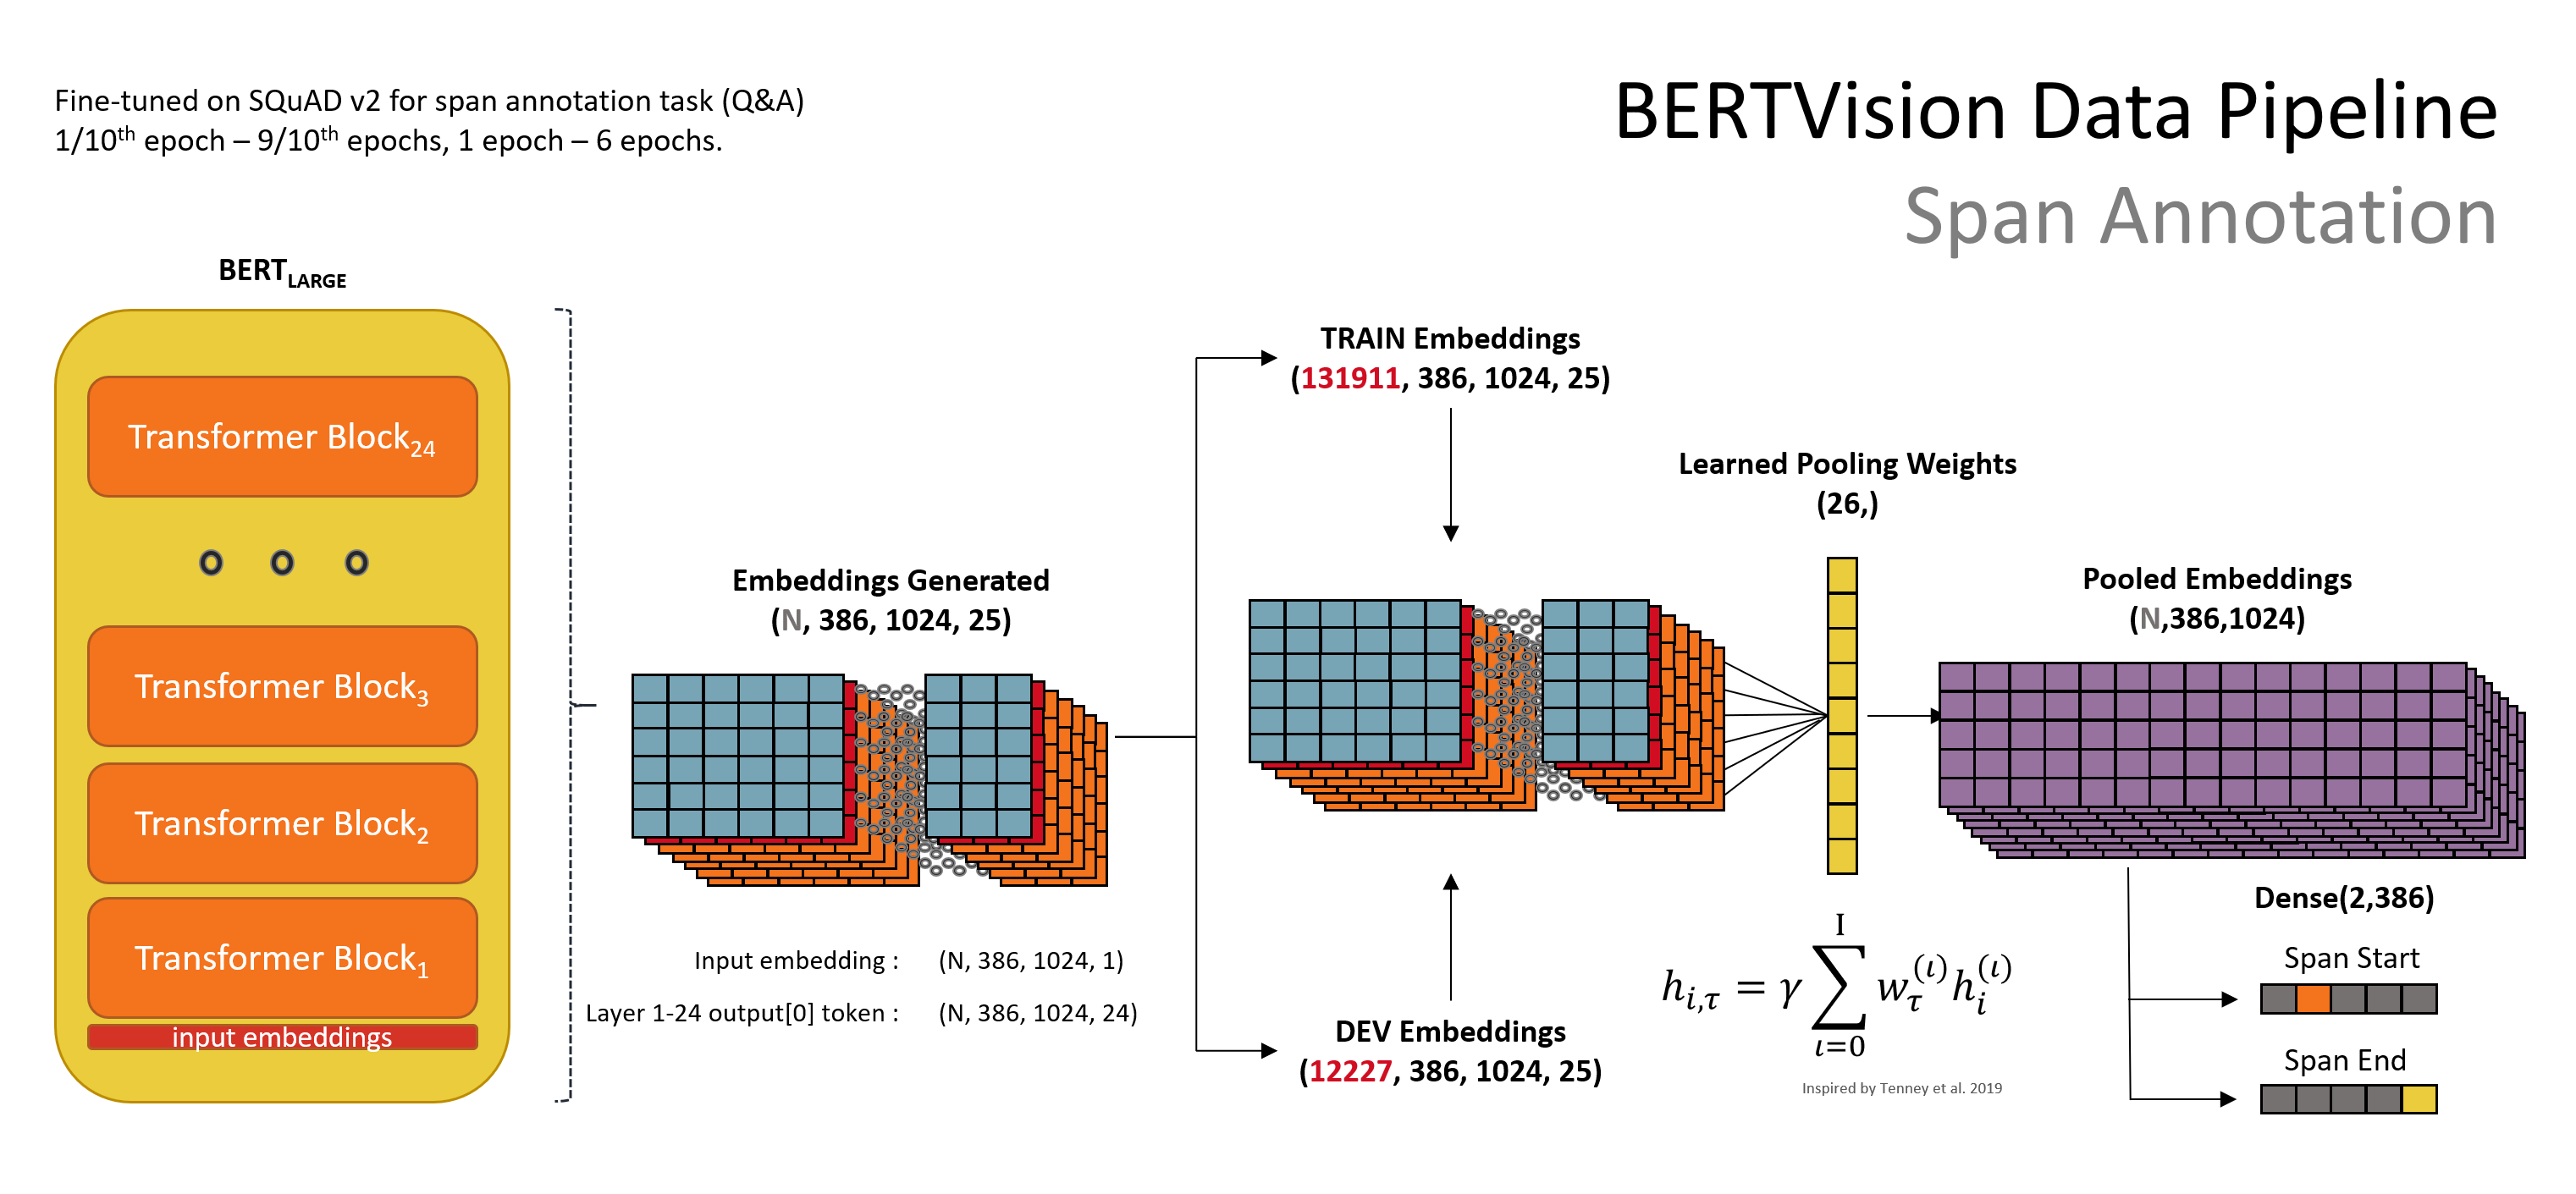
\includegraphics[width=\textwidth]{images/Data_Pipeline_Span_Annotation.png}%
	\caption{BERTVision span annotation data pipeline}
	\label{apdx:bertvision_span_annotation_data_pipeline_graph}
\end{figure*}

\begin{figure*}[!h]
	\centering
	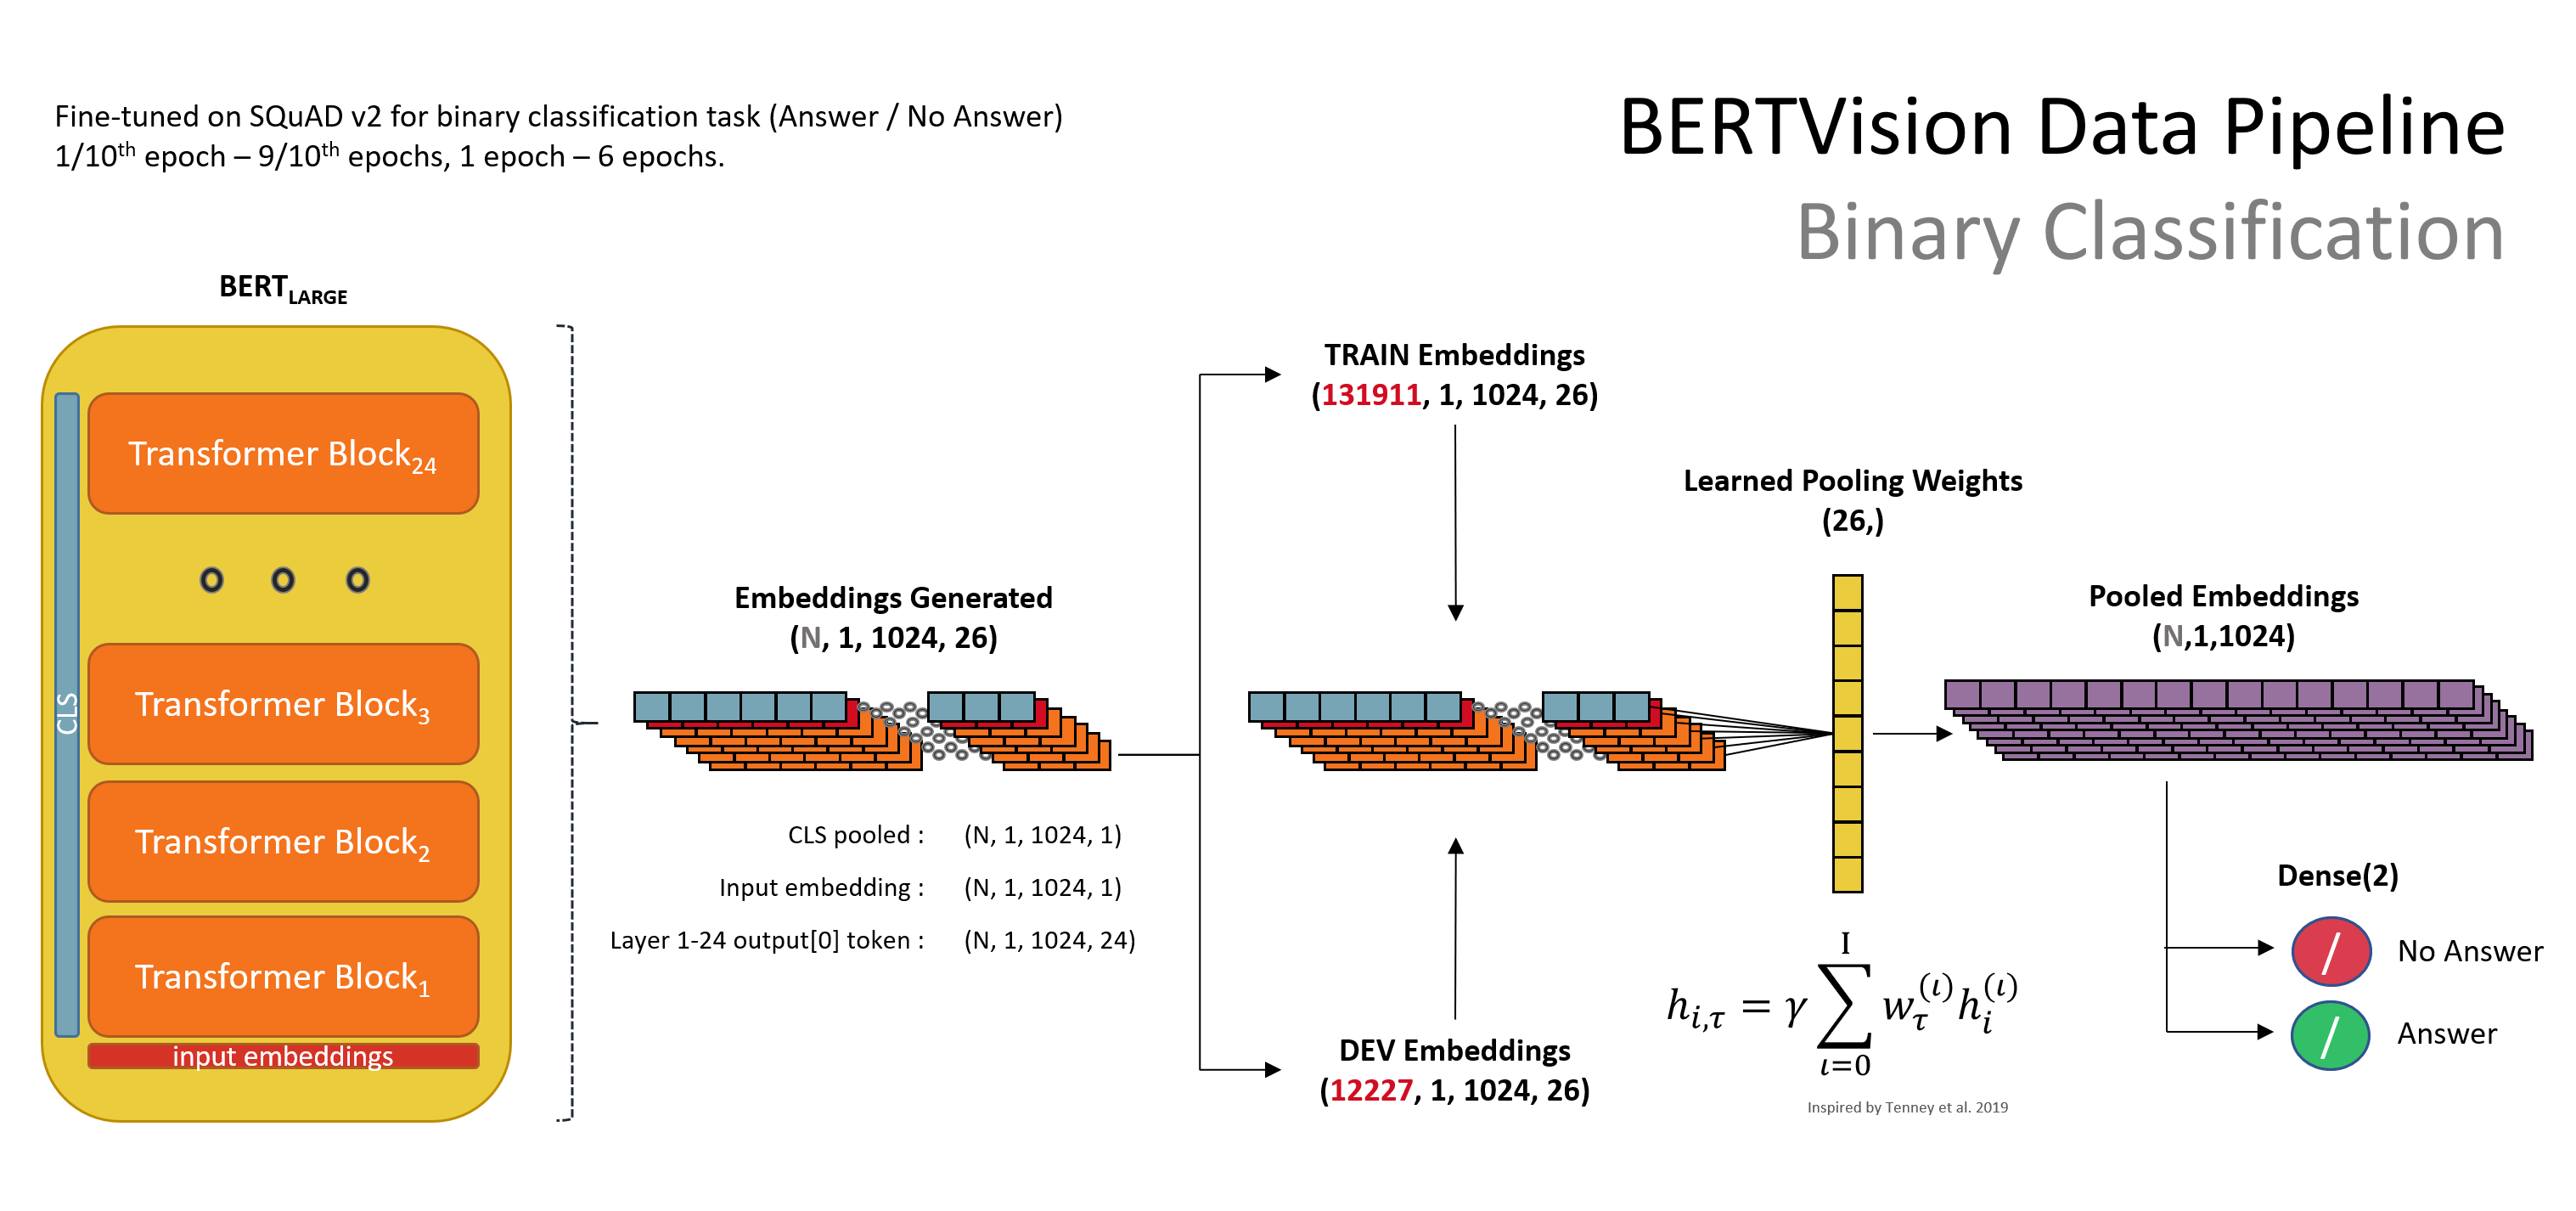
\includegraphics[width=\textwidth]{images/Data_Pipeline_Binary_Classification.png}%
	\caption{BERTVision classification data pipeline}
	\label{apdx:bertvision_classification_data_pipeline_graph}
\end{figure*}

\newpage

\subsection{Non-uniform weights}
\label{apdx:non-uniform}

Learned weights for learning pooling using the approach described in \cite{tenney-etal-2019-bert}. The model favors using later layers especially after layer 17. This is consistent with the observation in \cite{van_Aken_2019} that the last layers of BERT-base are much more accurate at supporting fact identification (which is the author’s proxy for span identification).



\end{document}
